\section{24H 挂机功能}

本集成工具通过实时确定游戏内状态,通过控制器向罗技软件下达命令,在游戏内执行相应的挂机动作。
因此,本集成工具支持游戏掉线以及因为各种原因离开房间(如房间长时间未开始游戏导致关闭、被强制踢出等)后重新创建房间继续挂机。
不过,需要注意的是本工具提供的掉线重连功能无法保证在所有情况下都能成功(如计算机断网、游戏维护等无法正常启动游戏的情形),但在大部分情况下能够正常工作。
掉线重连目的在于在发生掉线时尽最大努力恢复挂机。该功能受诸多因素影响,并非完全可靠,因此您不应过分依赖此功能。
挂机功能共分为两种:单人单件武器挂机(1 号功能)挂机及野房随机武器挂机(2 号功能)。
1 号功能可以搭配配件武器使用。2 号功能可以搭配特殊武器使用(如圣翼皓印)。
本集成工具支持选择 T 阵营或 CT 阵营角色。通关失败自动回合重置。
除灾变挂机外,本工具还可用于梦幻之星等荣誉图挂机。

使用挂机功能前,需要自行配置好游戏内各按钮的坐标位置以及挂机使用的武器列表。

\subsection{前提条件}

\begin{itemize}

\item 通过 TCGame 启动游戏,挂机期间需保证 TCGame 处于登录状态(不勾选“自动登录”的情况下,一段时间后登录信息会失效),否则无法正常使用掉线重连功能。如果您的电脑仅进行单账号挂机,则建议您在 TCGame 中勾选“自动登录”,这样每隔一段时间登录信息就会刷新。

\item \textbf{\color{red}强烈建议}将游戏设置为窗口化运行,全屏运行效果尚未测试过。

\item 确保 Lua 脚本文件正确保存并运行。

\item 运行控制器。

\item 运行 GamingTool.exe。

\end{itemize}

游戏启动进入大厅界面后(图 \ref{ch2fig-before-make-borderless}),按 \lstinline{Ctrl} \lstinline{Alt} \lstinline{B} 使用 GamingTool 无边框窗口化功能去除游戏窗口边框(图 \ref{ch2fig-after-make-borderless},同时还会将游戏窗口置于屏幕中央),如不去除边框,将可能导致挂机时使用的游戏按钮坐标不准确(例如,窗口位置被意外地移动)。

\begin{figure}
    \Centering
    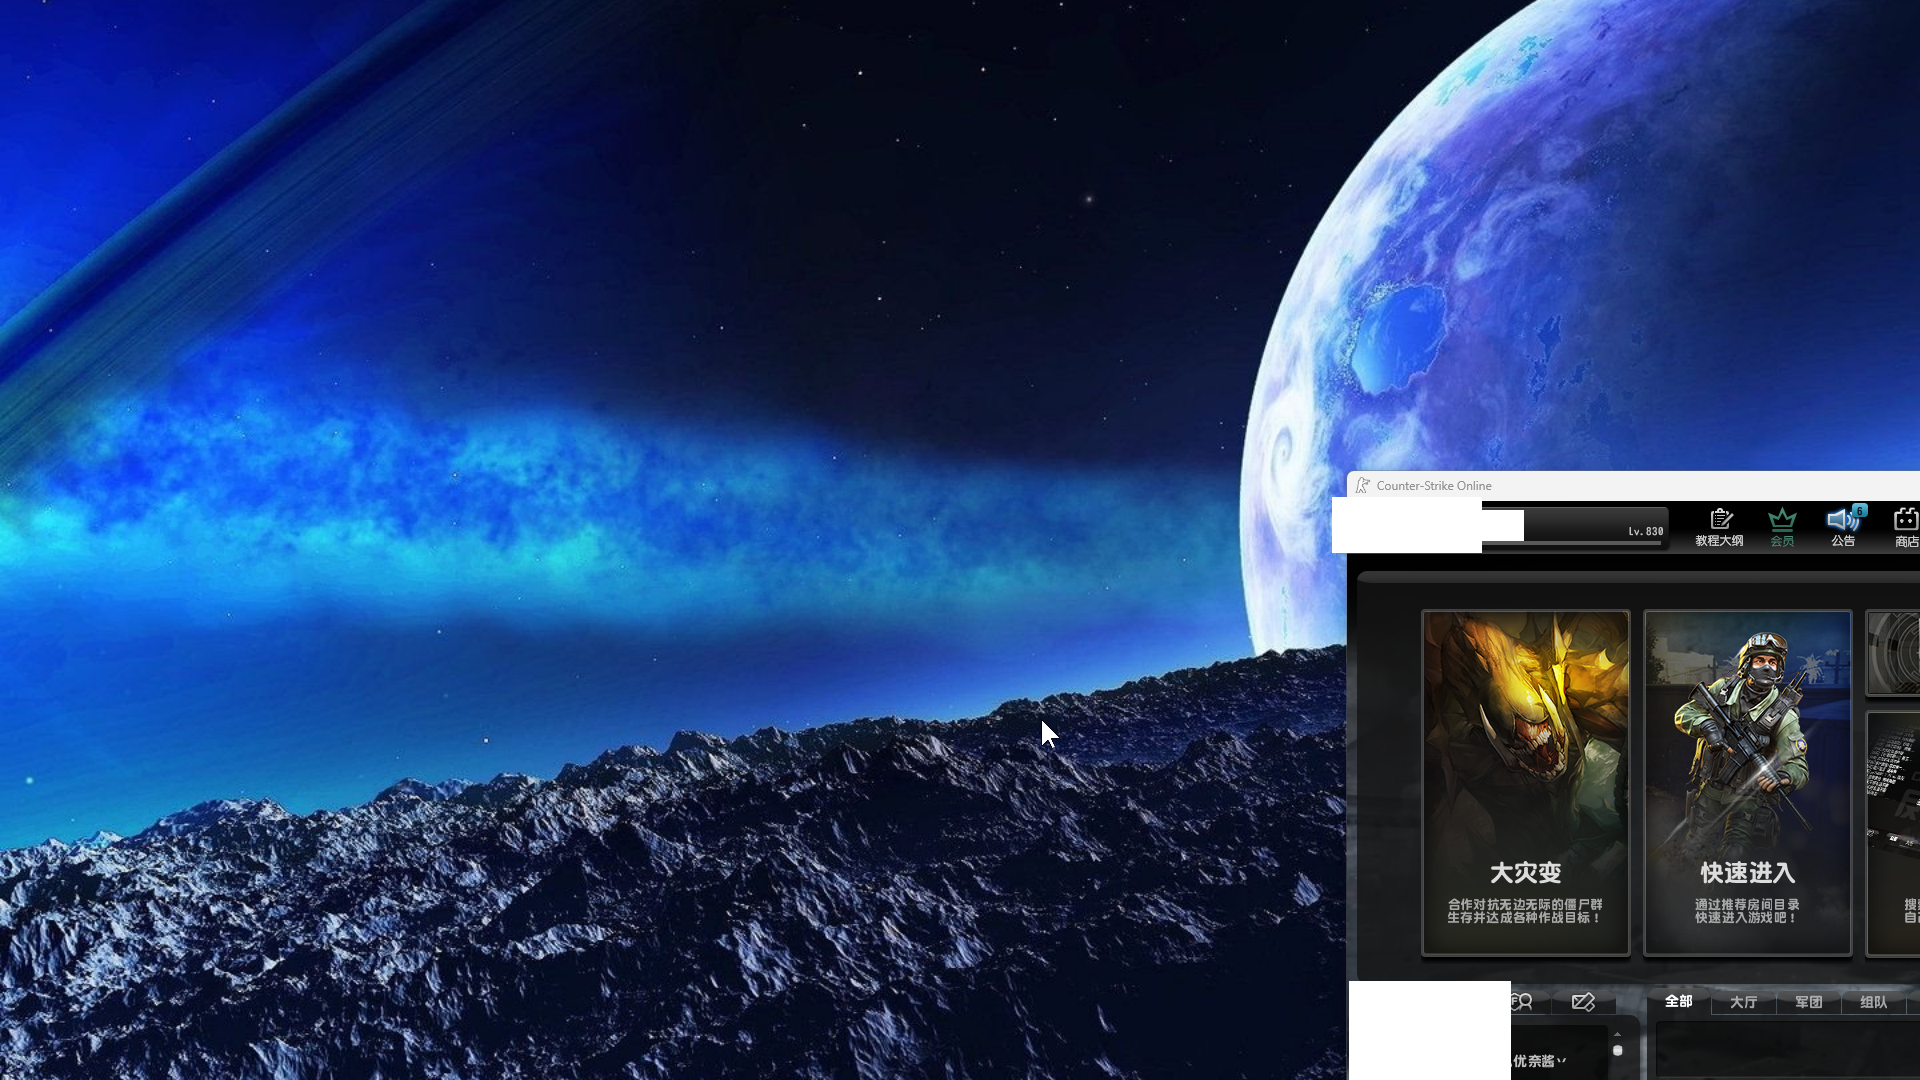
\includegraphics[width=\textwidth]{docs/assets/before-make-borderless.png}
    \caption{无边框窗口化前(窗口可随意移动)}
    \label{ch2fig-before-make-borderless}
\end{figure}

\begin{figure}
    \Centering
    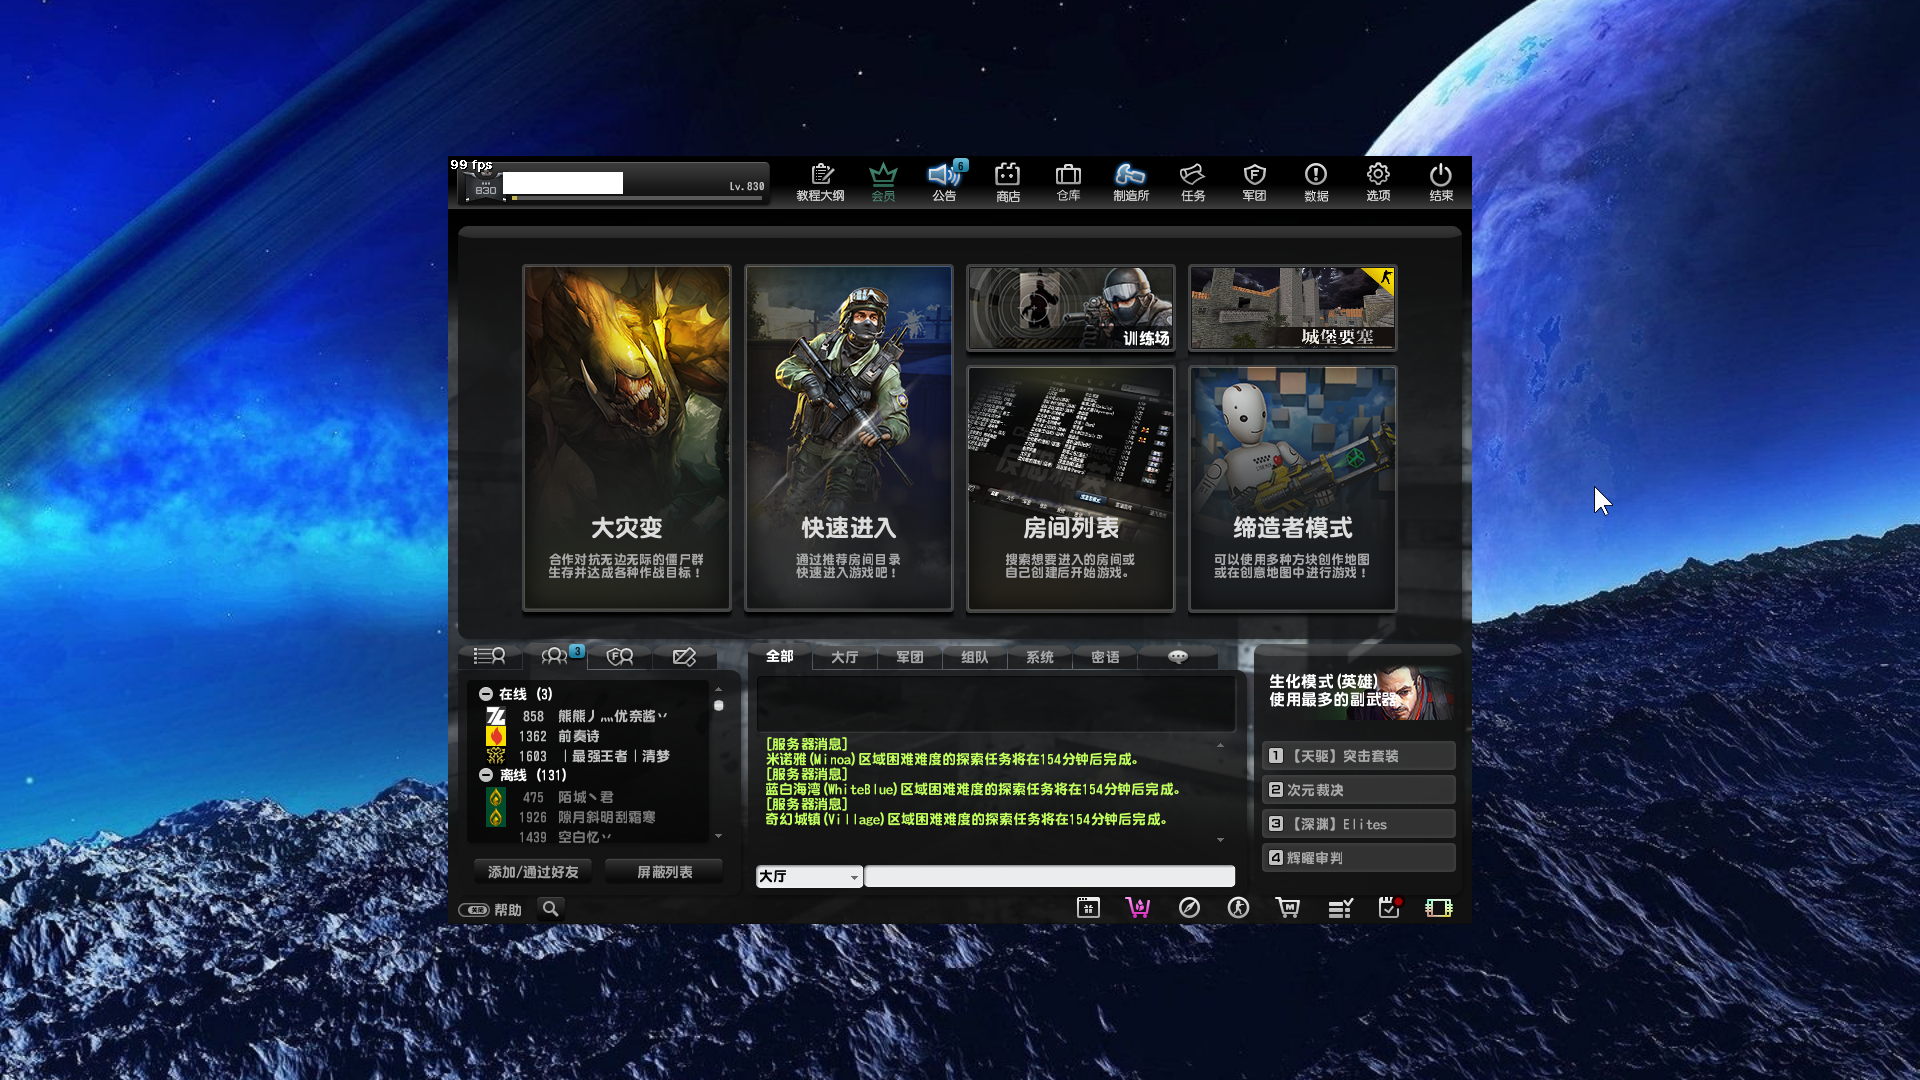
\includegraphics[width=\textwidth]{docs/assets/after-make-borderless.png}
    \caption{无边框窗口化后(窗口居中、标题栏去除、不可随意移动)}
    \label{ch2fig-after-make-borderless}
\end{figure}

有关 GamingTool 更多使用方法,参考 \href{https://gitee.com/silver1867/gaming-tool}{GamingTool 项目链接}。

\subsection{通用设置}

将控制器调到模式 5 进行坐标定位。

使用记事本打开 \lstinline{lua} 目录下的 \lstinline{Setting.lua} 文件,本文件存放所有游戏内按钮的屏幕坐标位置,所有的坐标均通过 5 模式坐标定位功能确定。
其中,\lstinline{NAME_X}(\lstinline{NAME} 为某个坐标名称)表示横坐标,\lstinline{NAME_Y} 表示纵坐标。

下面,详细介绍 \lstinline{Setting.lua} 文件中各个变量的含义,使用模式 5 坐标定位功能耐心配置即可。

\textbf{\color{red}注意:配置文件修改后后,需要在罗技软件中重新导入并运行以使配置生效。}

\begin{figure}[H]
    \Centering
    \parbox[l]{\textwidth}{\lstinline{TIME_ZONE}:操作系统时区(图 \ref{ch2fig-os-timezone}),东半球为正数,西半球为负数。例如,中国处于东八区(UTC+08:00),则应将其设置为 8(默认配置,一般不需更改)。}
    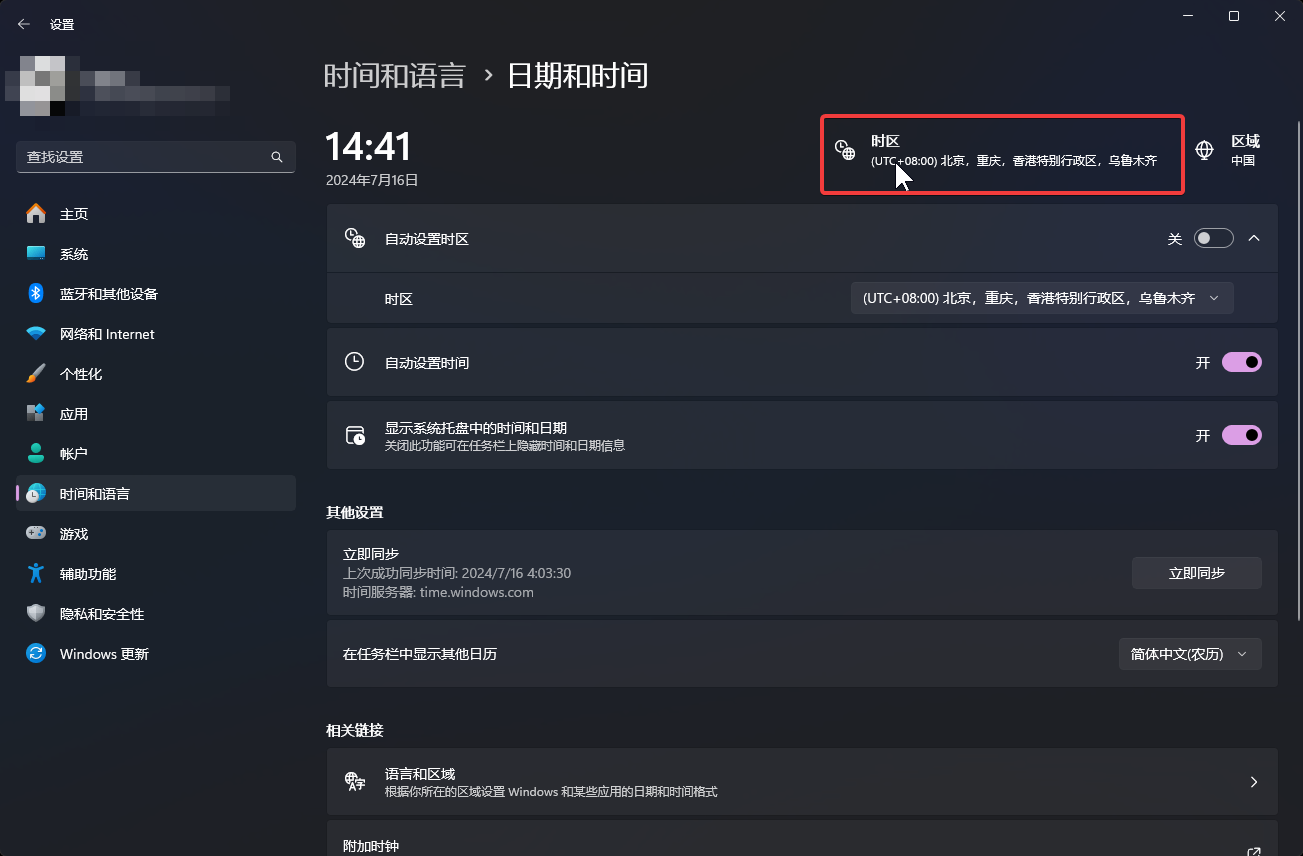
\includegraphics[width=\textwidth]{docs/assets/timezone}
    \caption{操作系统时区}
    \label{ch2fig-os-timezone}
\end{figure}


\begin{figure}[H]
    \Centering
    \parbox[l]{\textwidth}{\lstinline{HALL_ROOM_LIST_X}、\lstinline{ROOM_LIST_Y}:大厅房间列表选框的坐标(图 \ref{ch2fig-room-list})。}
    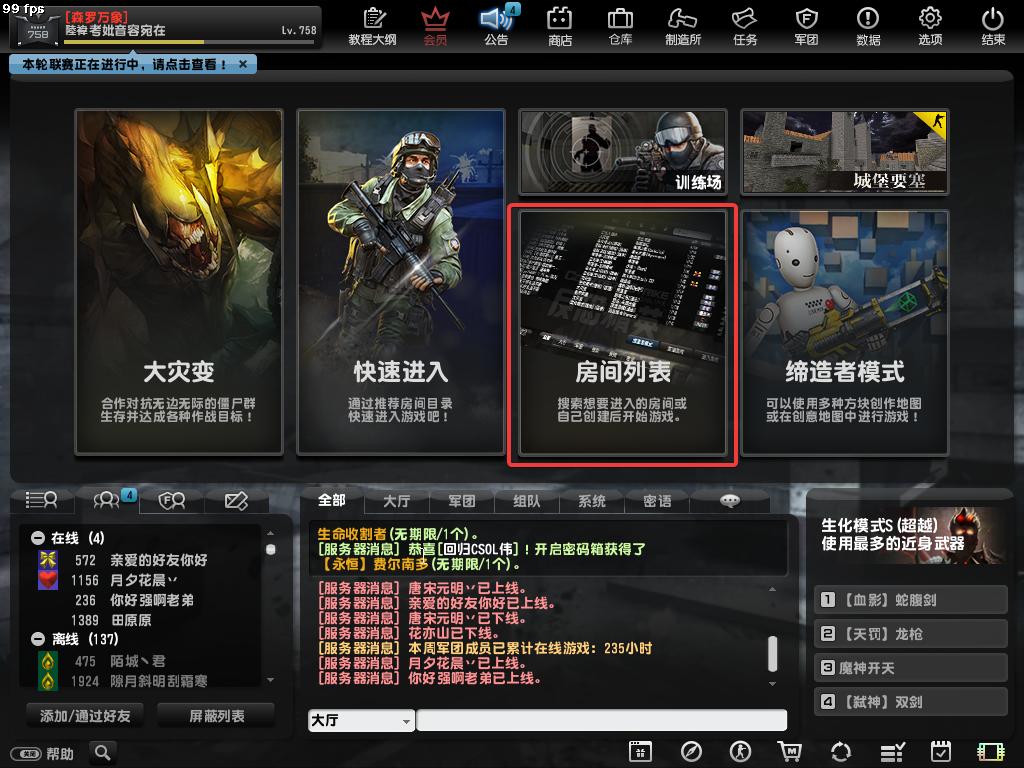
\includegraphics[width=\textwidth]{docs/assets/room_list}
    \caption{房间列表按钮}
    \label{ch2fig-room-list}
\end{figure}


\begin{figure}[H]
    \Centering
    \parbox[l]{\textwidth}{\lstinline{HALL_CREATE_ROOM_X}、\lstinline{HALL_CREATE_ROOM_Y}:大厅中的“新建房间”按钮坐标(图 \ref{ch2fig-create-room-0})。}
    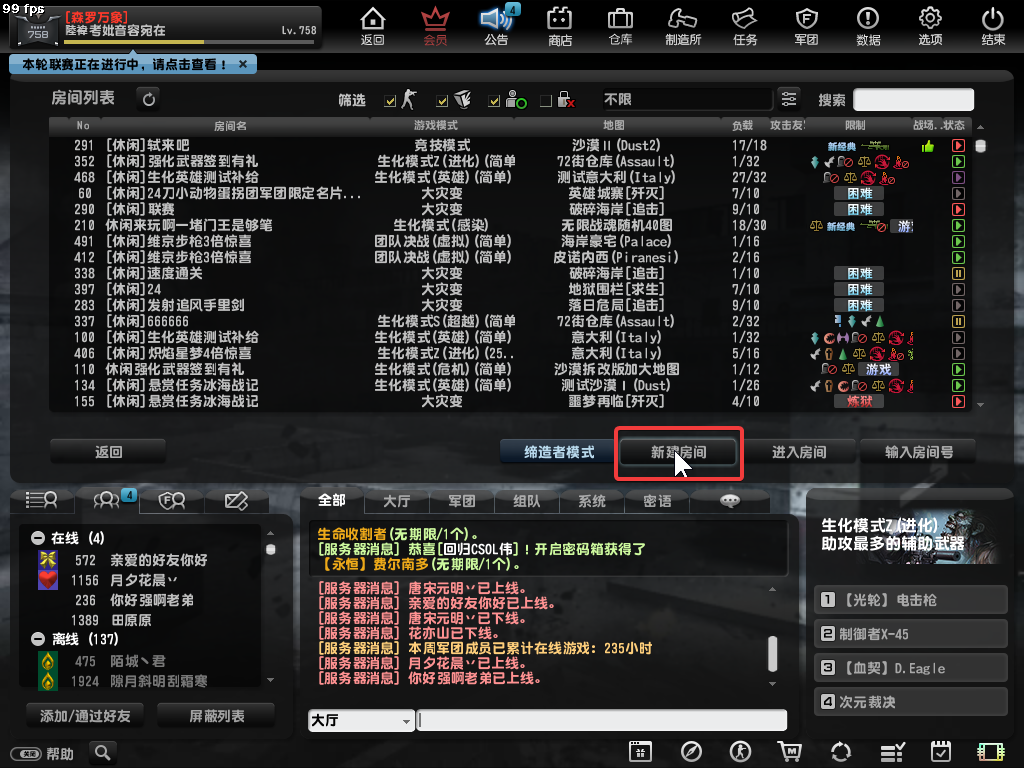
\includegraphics[width=\textwidth]{docs/assets/create_room_0}
    \caption{大厅中的“新建房间”按钮}
    \label{ch2fig-create-room-0}
\end{figure}


\begin{figure}[H]
    \Centering
    \parbox[l]{\textwidth}{\lstinline{HALL_BACK_X}、\lstinline{HALL_BACK_Y}:大厅房间列表界面中的“返回”按钮坐标(图 \ref{ch2fig-hall-back})。}
    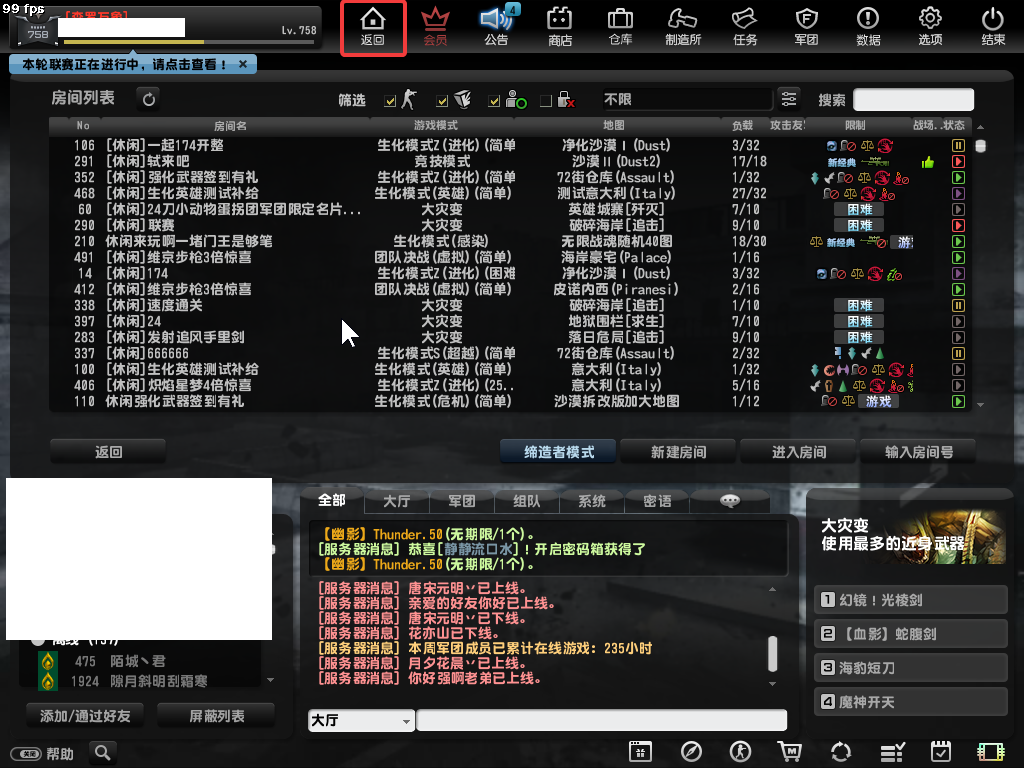
\includegraphics[width=\textwidth]{docs/assets/hall_back}
    \caption{大厅房间列表界面中的“返回”按钮}
    \label{ch2fig-hall-back}
\end{figure}


\begin{figure}[H]
    \Centering
    \parbox[l]{\textwidth}{\lstinline{GAME_MODE_X}、\lstinline{GAME_MODE_Y}:点击大厅房间列表界面的“创建游戏”按钮后,弹出窗口中的“游戏模式”选框坐标(图 \ref{ch2fig-game-mode})。}
    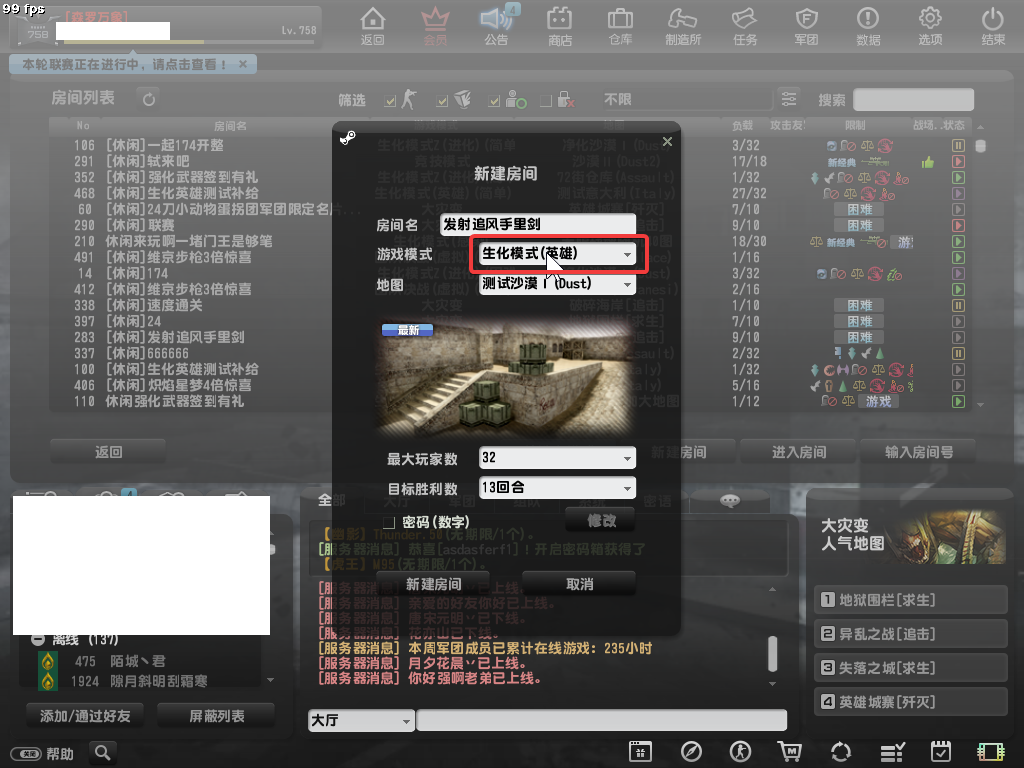
\includegraphics[width=\textwidth]{docs/assets/game_mode.png}
    \caption{“游戏模式”选框}
    \label{ch2fig-game-mode}
\end{figure}


\begin{figure}[H]
    \Centering
    \parbox[l]{\textwidth}{\lstinline{ZOMBIE_SECNARIO_MODE_X}、\lstinline{ZOMBIE_SCENARIO_MODE_Y}:“大灾变”模式选框(图 \ref{ch2fig-zombie-scenario},亦可根据自身需要选择其他模式,如娱乐模式)。}
    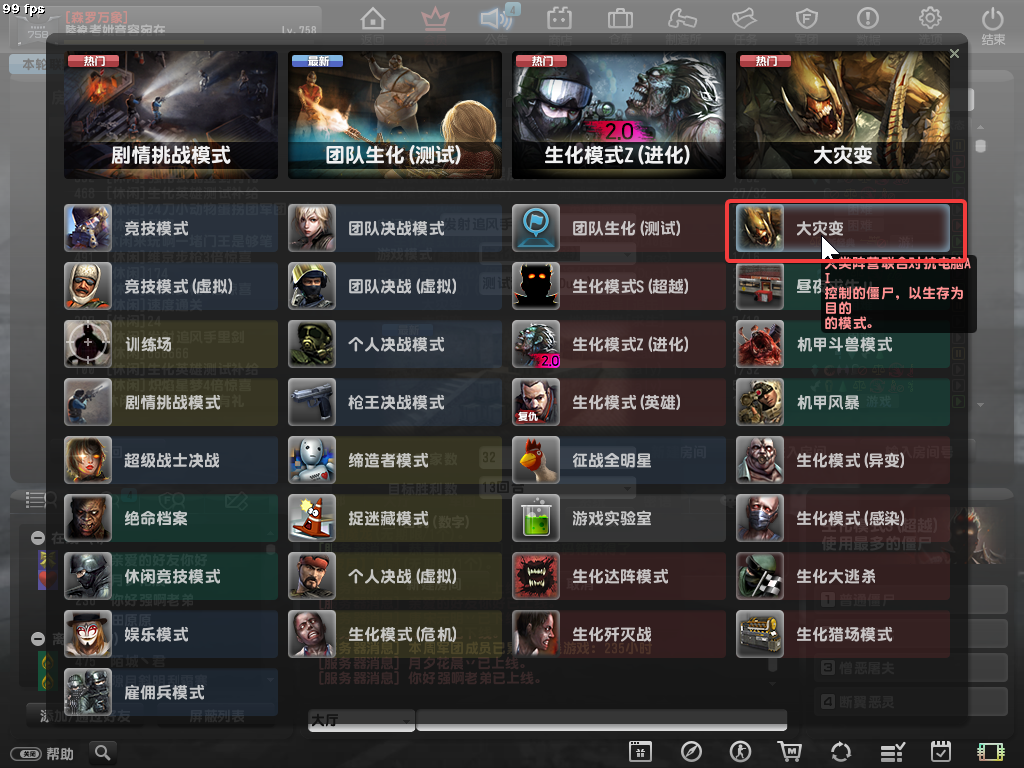
\includegraphics[width=\textwidth]{docs/assets/zombie_scenario.png}
    \caption{选择挂机模式}
    \label{ch2fig-zombie-scenario}
\end{figure}


\begin{figure}[H]
    \Centering
    \parbox[l]{\textwidth}{\lstinline{MAP_CHOOSE_LEFT_SCROLL_X}、\lstinline{MAP_CHOOSE_LEFT_SCROLL_Y}:地图选择界面中的向左滚动按钮(图 \ref{ch2fig-left-scroll})。}
    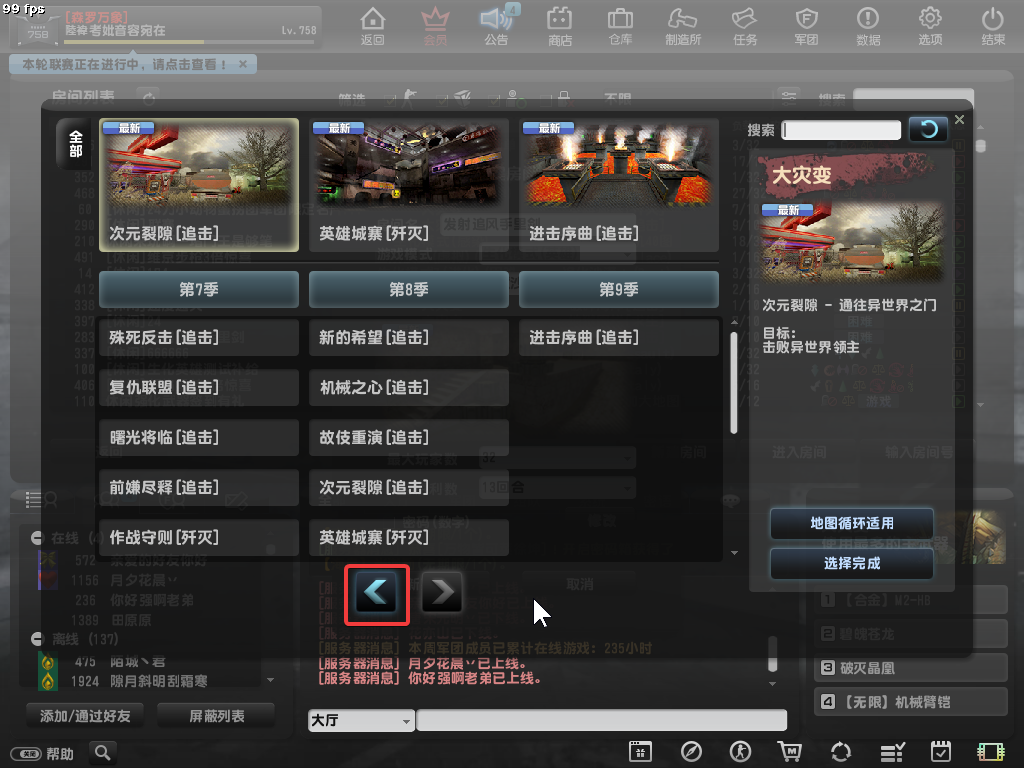
\includegraphics[width=\textwidth]{docs/assets/left_scroll.png}
    \caption{向左滚动按钮}
    \label{ch2fig-left-scroll}
\end{figure}

\begin{figure}[H]
    \Centering
    \parbox[l]{\textwidth}{\lstinline{MAP_TRAP_X}、\lstinline{MAP_TRAP_Y}:“地狱围栏”地图按钮坐标(图 \ref{ch2fig-map-trap},亦可根据自身需要选择其他地图,如用于刷梦幻之星的铁笼蝎斗)。}
    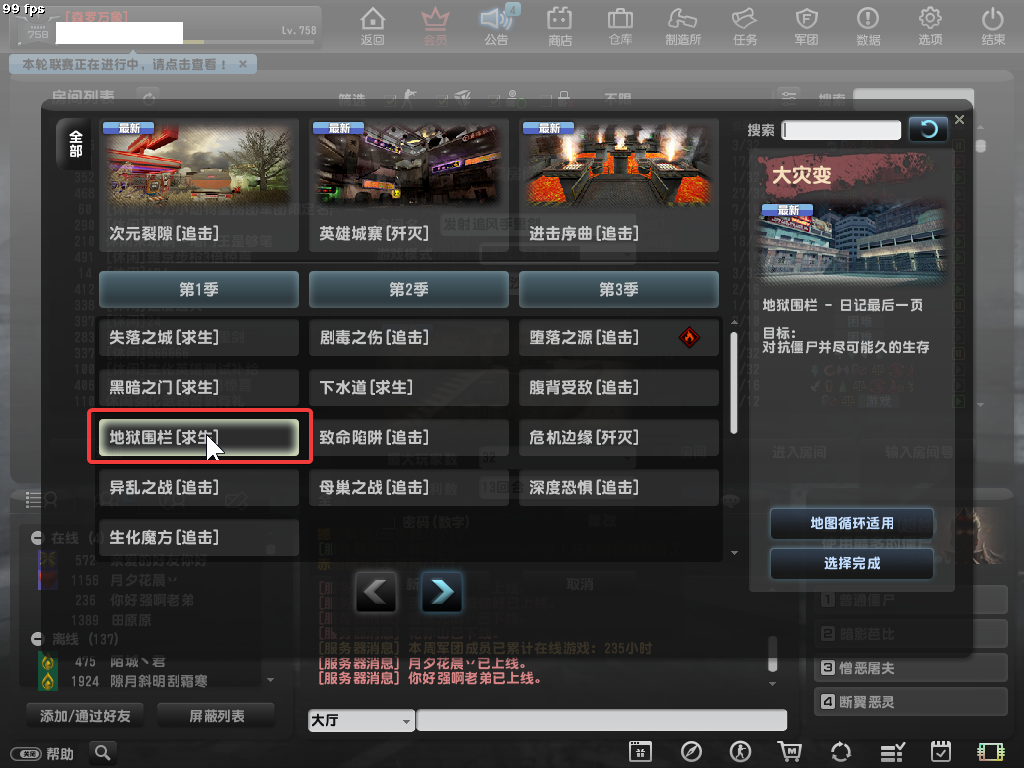
\includegraphics[width=\textwidth]{docs/assets/map_trap.png}
    \caption{默认挂机的地图}
    \label{ch2fig-map-trap}
\end{figure}

\begin{figure}[H]
    \Centering
    \parbox[l]{\textwidth}{\lstinline{FINISH_CHOOSE_X}、\lstinline{FINISH_CHOOSE_Y}:“选择完成”按钮坐标(图 \ref{ch2fig-finish-choose})。}
    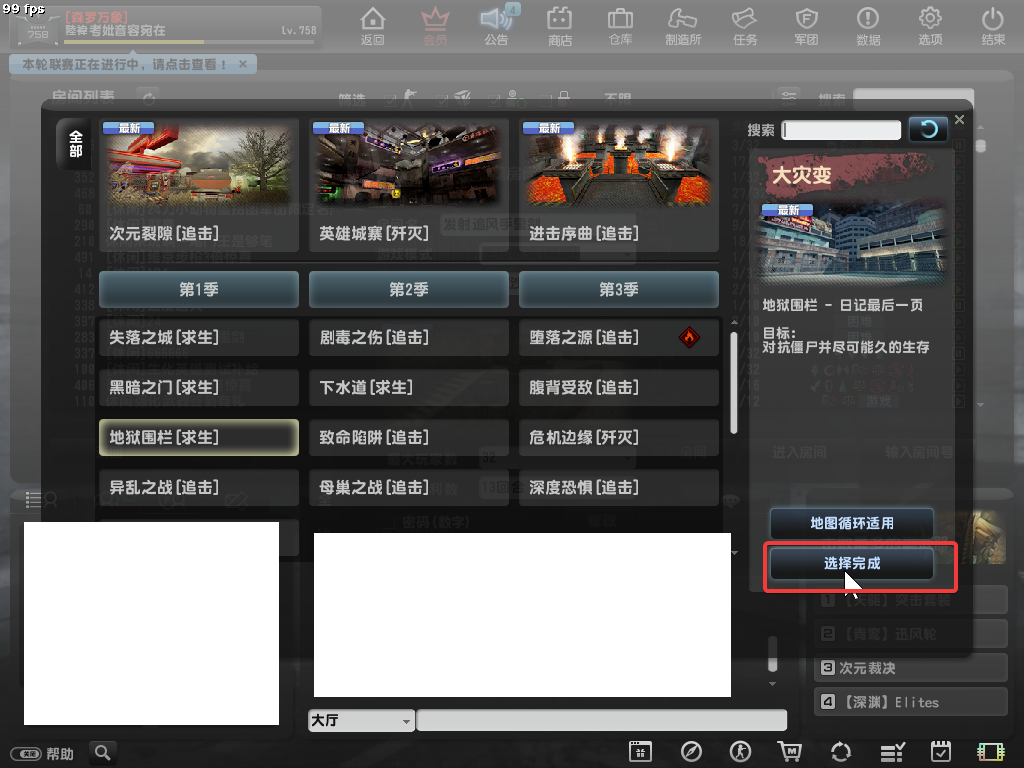
\includegraphics[width=\textwidth]{docs/assets/finish_choose.png}
    \caption{“选择完成”按钮}
    \label{ch2fig-finish-choose}
\end{figure}

\begin{figure}[H]
    \Centering
    \parbox[l]{\textwidth}{\lstinline{GAME_DIFFICULTY_X}、\lstinline{GAME_DIFFICULTY_Y}:“游戏难度”选框坐标(图 \ref{ch2fig-choose-difficulty})。}
    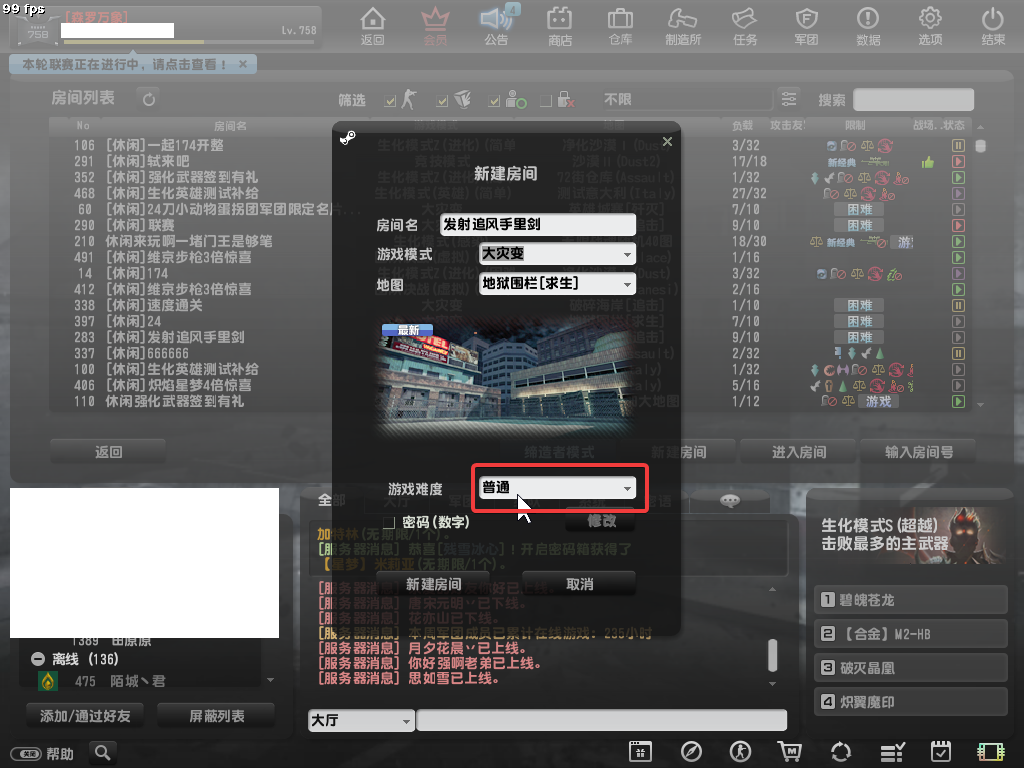
\includegraphics[width=\textwidth]{docs/assets/choose_difficulty.png}
    \caption{“游戏难度”按钮}
    \label{ch2fig-choose-difficulty}
\end{figure}

\begin{figure}[H]
    \Centering
    \parbox[l]{\textwidth}{\lstinline{GAME_DIFFICULTY_OPTION_X}、\lstinline{GAME_DIFFICULTY_OPTION_Y}:游戏难度选项坐标(图 \ref{ch2fig-difficulty-option}),建议设置为“困难”。对于条件一般的账号,可选择“普通”,具体视自身情况确定。}
    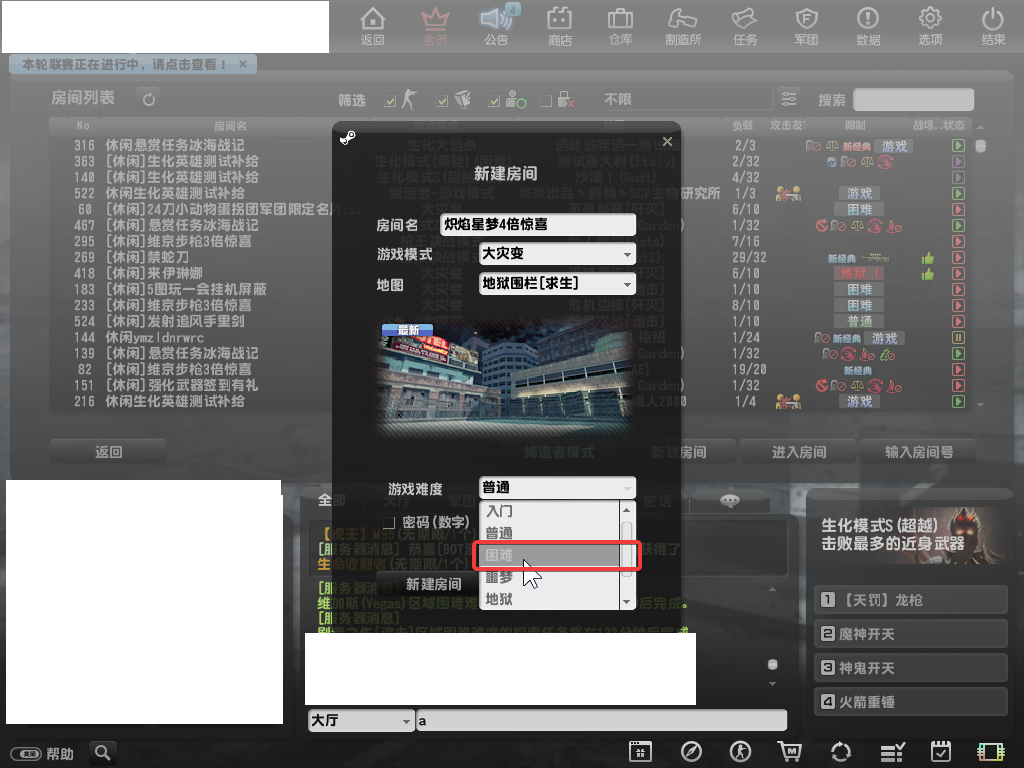
\includegraphics[width=\textwidth]{docs/assets/difficulty_option.png}
    \caption{游戏难度选项}
    \label{ch2fig-difficulty-option}
\end{figure}

\begin{figure}[H]
    \Centering
    \parbox[l]{\textwidth}{\lstinline{CREATE_ROOM_X}、\lstinline{CREATE_ROOM_Y}:“新建房间”按钮坐标(图 \ref{ch2fig-create-room-1})。}
    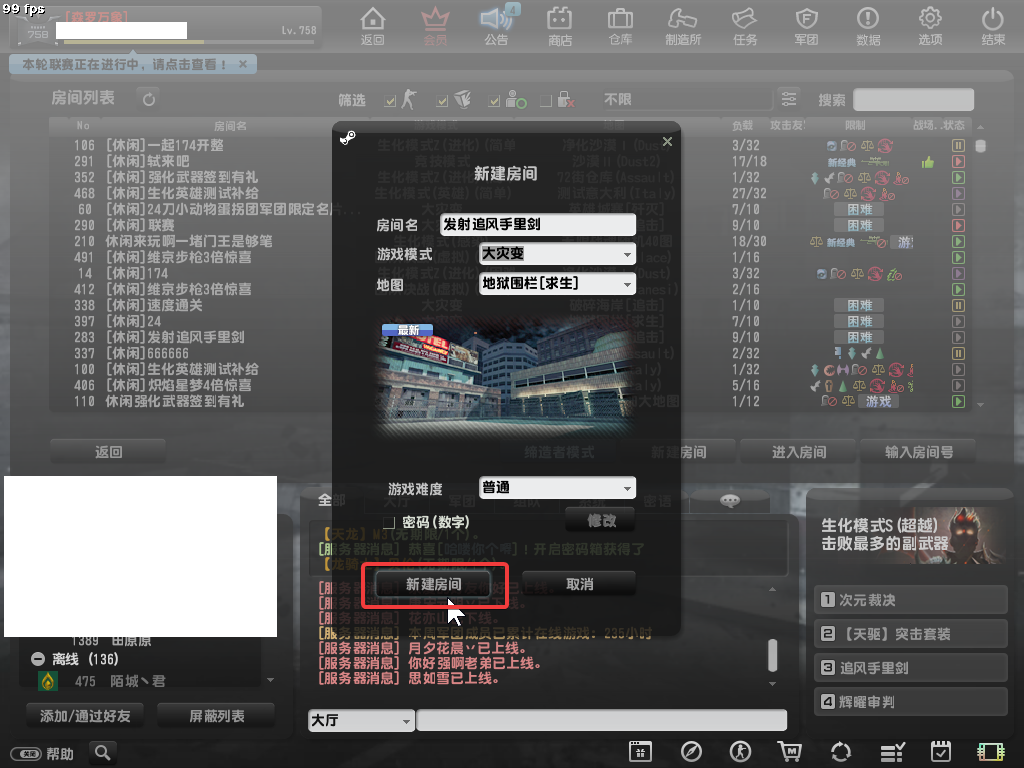
\includegraphics[width=\textwidth]{docs/assets/create_room_1.png}
    \caption{“新建房间”按钮}
    \label{ch2fig-create-room-1}
\end{figure}

\begin{figure}[H]
    \Centering
    \parbox[l]{\textwidth}{\lstinline{ROOM_GAME_START_X}、\lstinline{ROOM_GAME_START_Y}:房间内的“开始游戏”按钮坐标(图 \ref{ch2fig-start-game})。}
    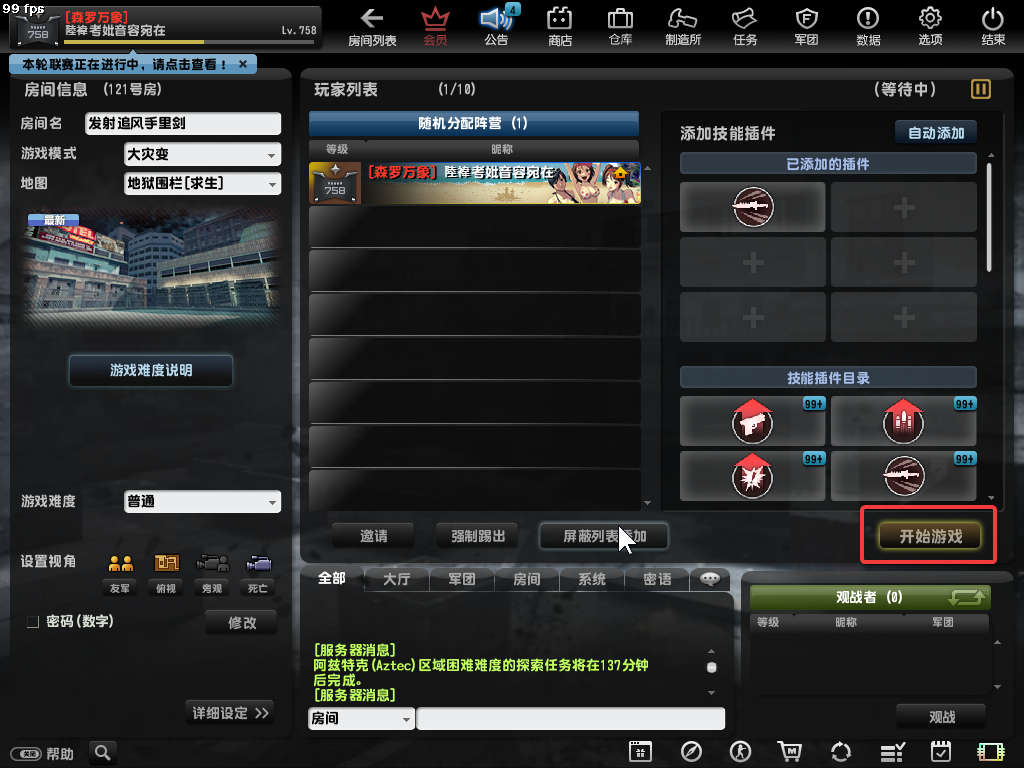
\includegraphics[width=\textwidth]{docs/assets/start_game.png}
    \caption{“开始游戏”按钮}
    \label{ch2fig-start-game}
\end{figure}

\lstinline{CHOOSE_T_CLASS}:是否选择 T 阵营角色。如要选择 T 阵营角色,则将其设置为 \lstinline{true};若要选择 CT 阵营角色,则将其置为 \lstinline{false}。

\begin{figure}[H]
    \Centering
    \parbox[l]{\textwidth}{\lstinline{CHOOSE_T_CLASS_X}、\lstinline{CHOOSE_T_CLASS_Y}:切换到 T 阵营选择界面的按钮坐标(图 \ref{ch2fig-choose-t-class})。只有在您需要选择 T 阵营角色时(\lstinline{CHOOSE_T_CLASS} 为 \lstinline{true}),才会使用到该坐标。}
    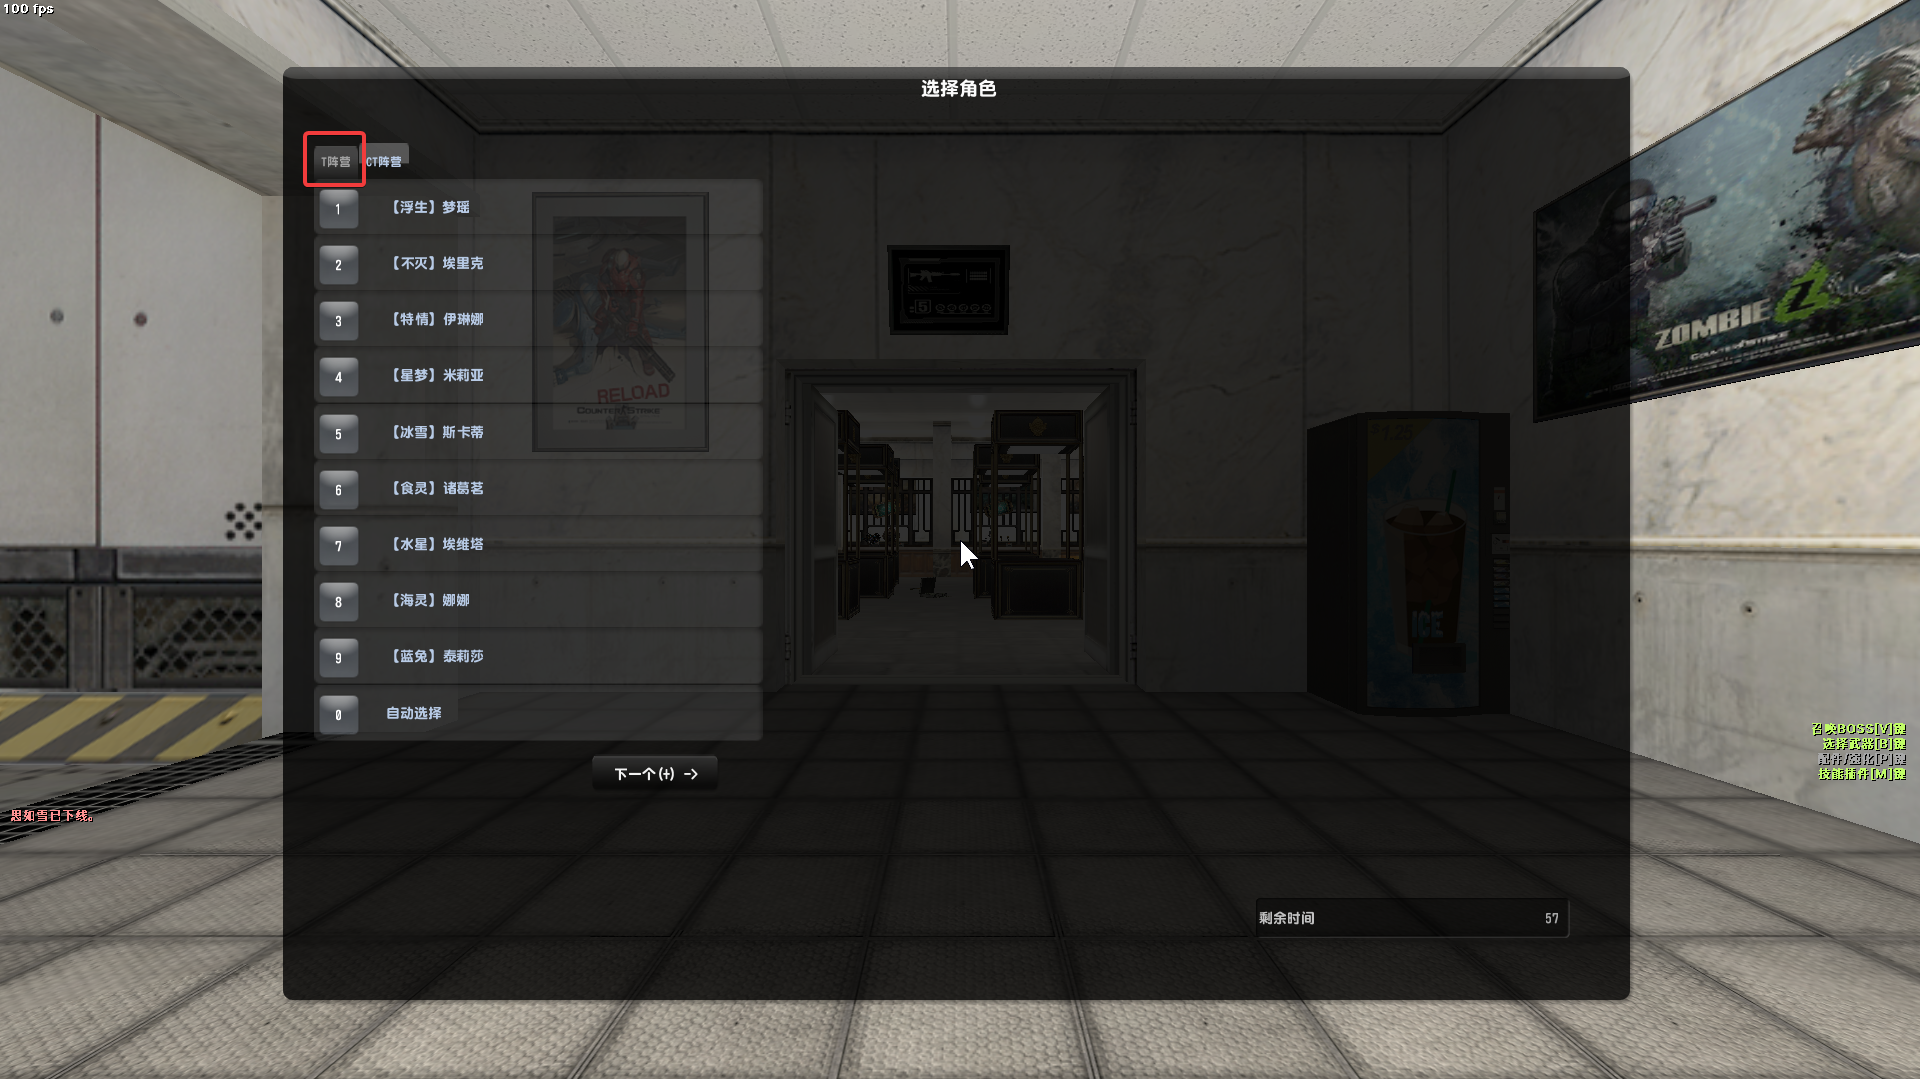
\includegraphics[width=\textwidth]{docs/assets/choose_T_class.png}
    \caption{“选择 T 阵营”按钮}
    \label{ch2fig-choose-t-class}
\end{figure}

\lstinline{CLASS_OPTION}:角色选项,取值范围为 0 \textasciitilde 9 范围内的整数。

\begin{figure}[H]
    \Centering
    \parbox[l]{\textwidth}{\lstinline{ZS_GAME_ESC_MENU_CANCEL_X}、\lstinline{ZS_GAME_ESC_MENU_CANCEL_Y}:“大灾变”模式下按 \lstinline{ESC} 后弹出的窗口中的“取消”按钮(图 \ref{ch2fig-zs-esc-cancel})。\textbf{\color{red}注意:大灾变模式中取消按钮的位置与其他模式不同。}}
    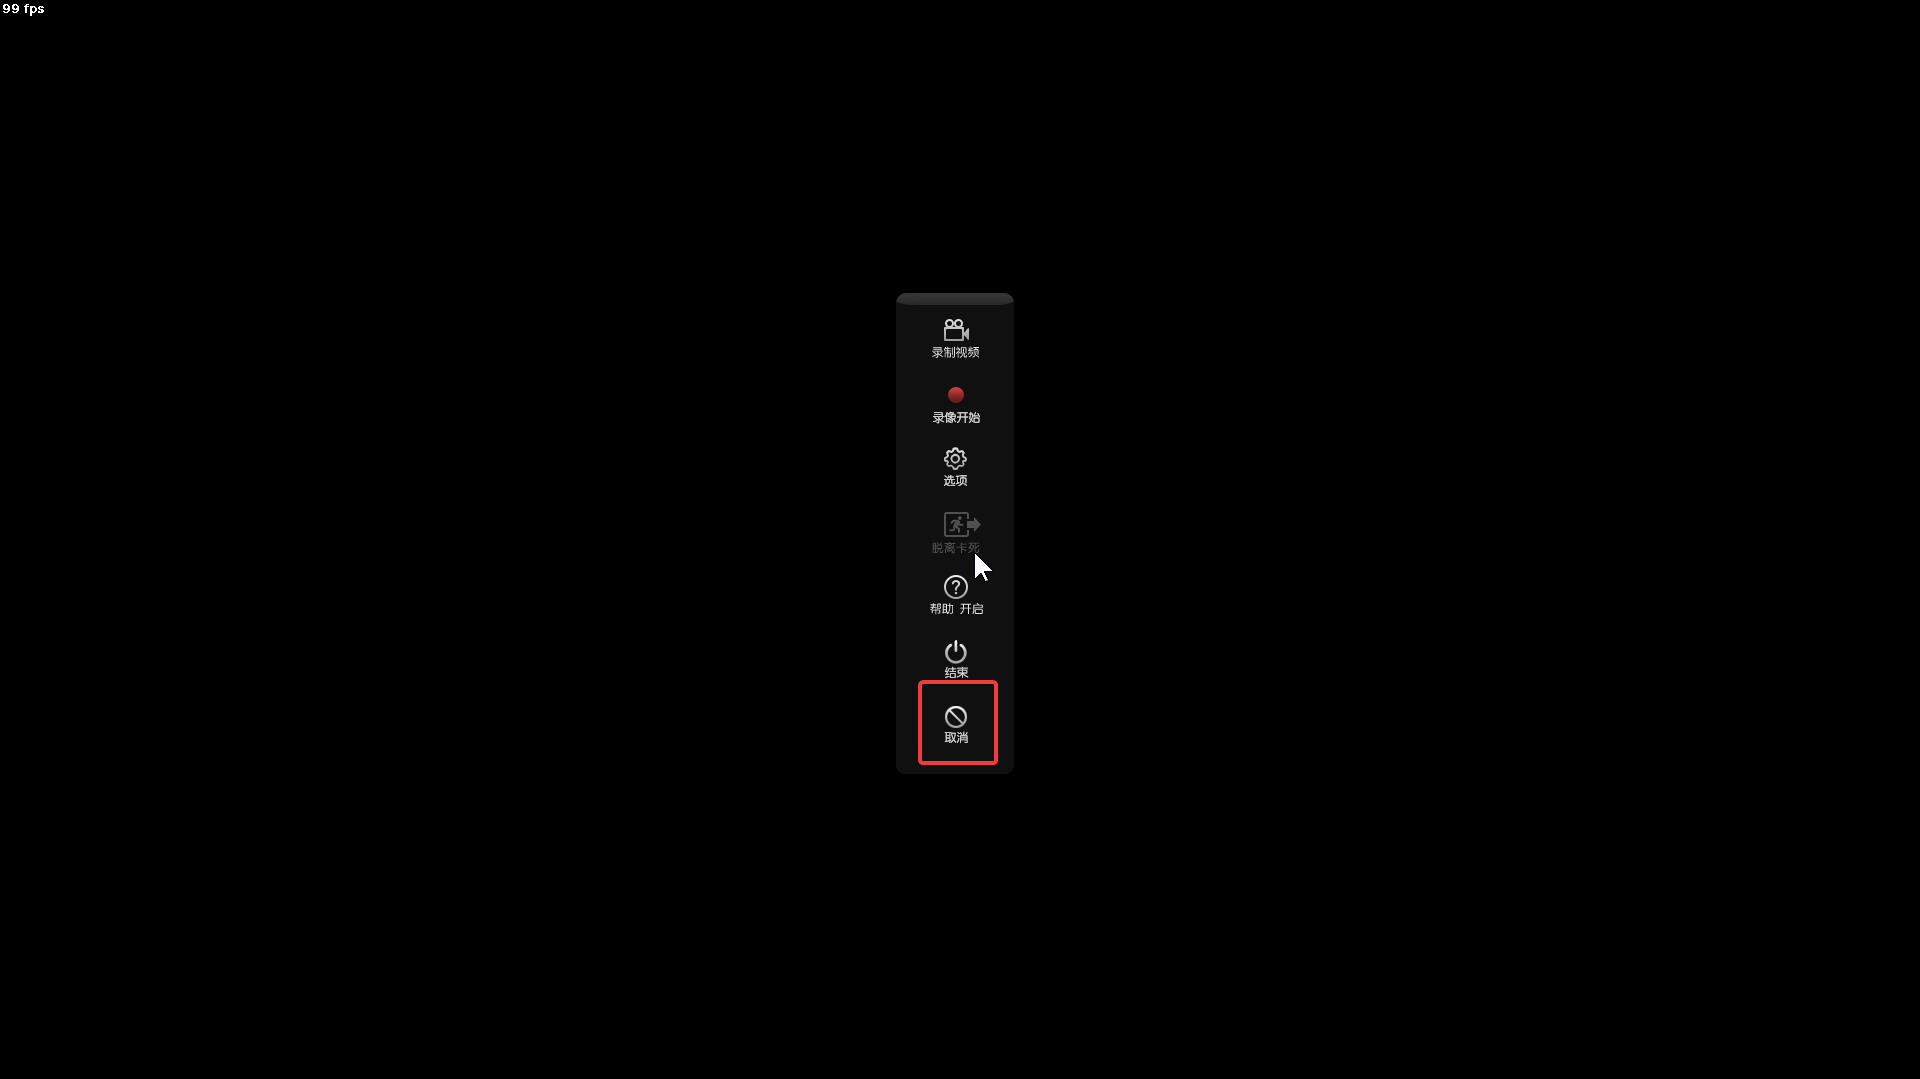
\includegraphics[width=\textwidth]{docs/assets/zs_esc_cancel.png}
    \caption{“大灾变”模式按下 \lstinline{ESC} 后的取消按钮}
    \label{ch2fig-zs-esc-cancel}
\end{figure}

\begin{figure}[H]
    \Centering
    \parbox[l]{\textwidth}{\lstinline{GAME_INSUFFICIENT_FUNDS_CONFIRM_X}、\lstinline{GAME_INSUFFICIENT_FUNDS_CONFIRM_Y}:“资金不足,无法购买”对话框中的“确认”按钮坐标(图 \ref{ch2fig-game-insuff-funds-confirm})。}
    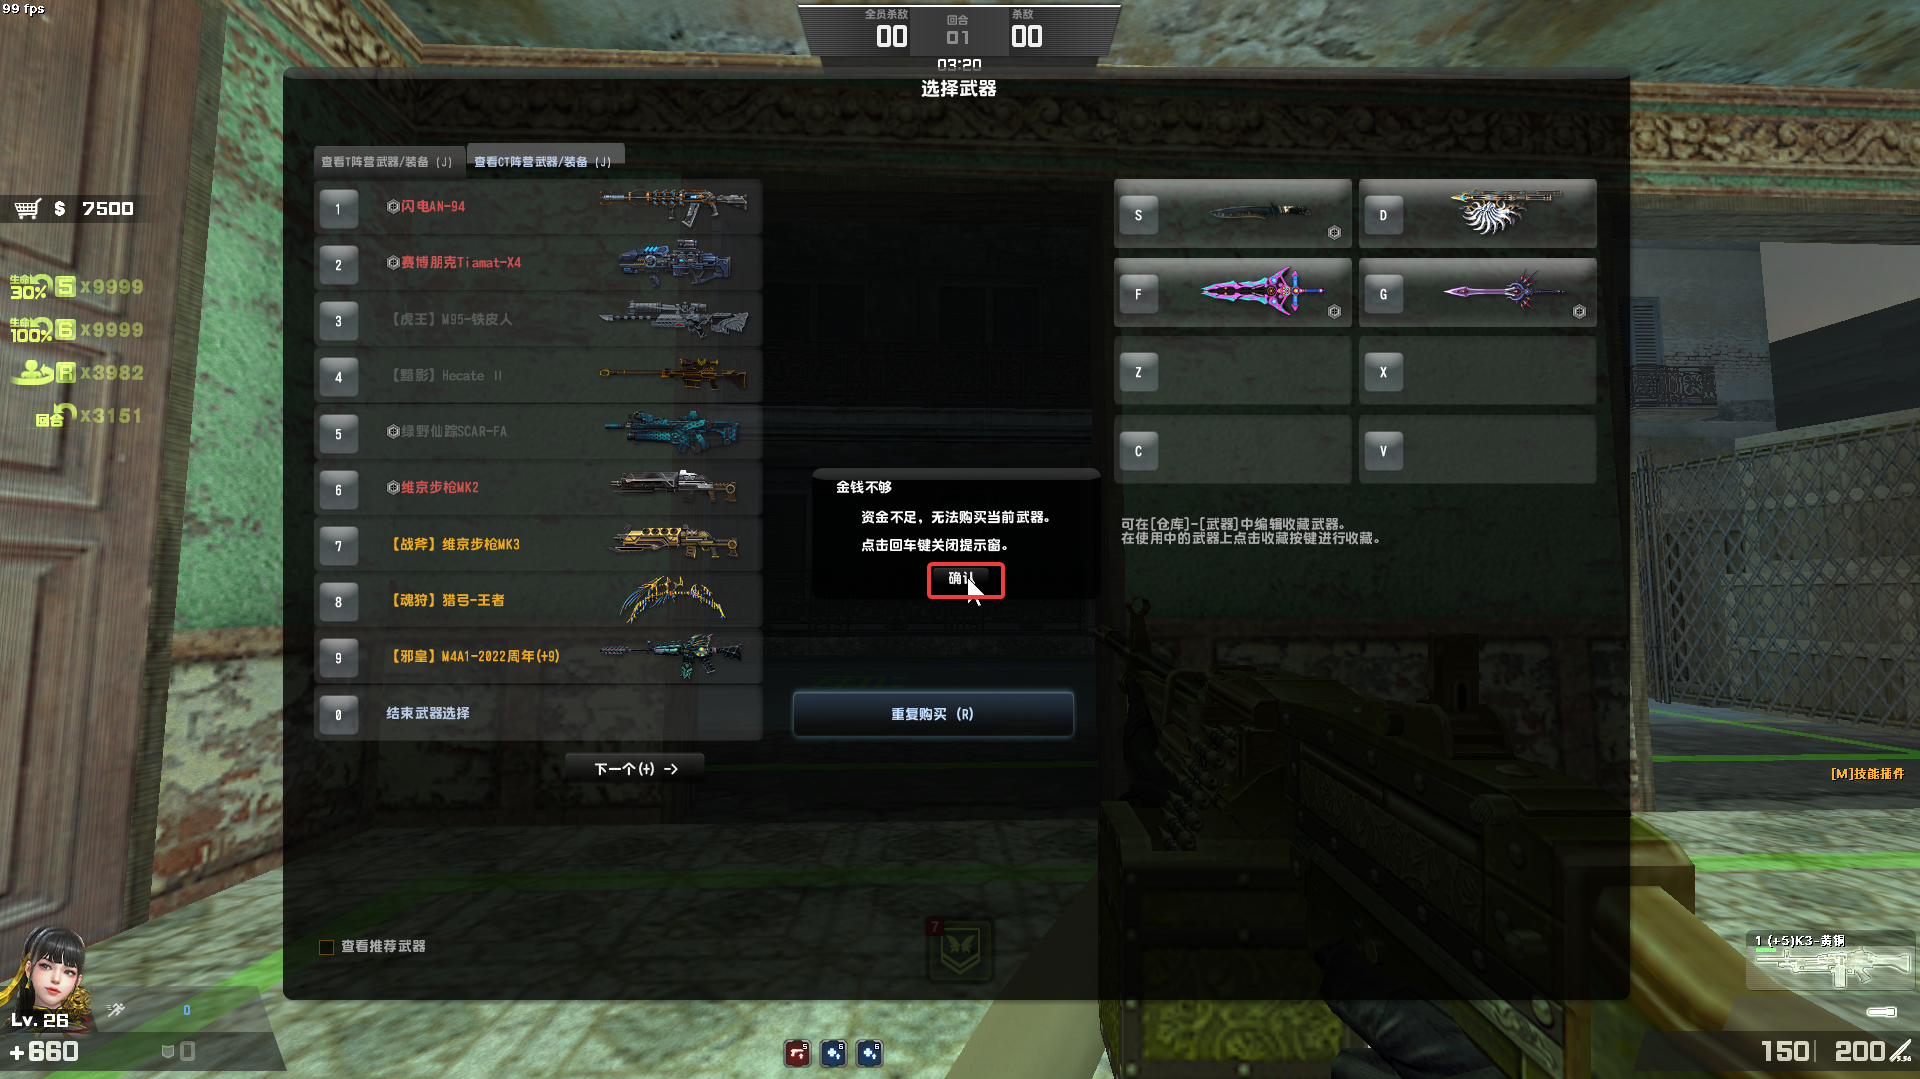
\includegraphics[width=\textwidth]{docs/assets/game_insuff_funds_confirm.png}
    \caption{“资金不足”确认按钮}
    \label{ch2fig-game-insuff-funds-confirm}
\end{figure}

\begin{figure}[H]
    \Centering
    \parbox[l]{\textwidth}{\lstinline{GAME_DEAD_PURCHASE_MENU_REBUY_X}、\lstinline{GAME_DEAD_PURCHASE_MENU_REBUY_Y}:大灾变死亡后预购买菜单中的“重复购买”按钮(图 \ref{ch2fig-dead-purchase-rebuy})。}
    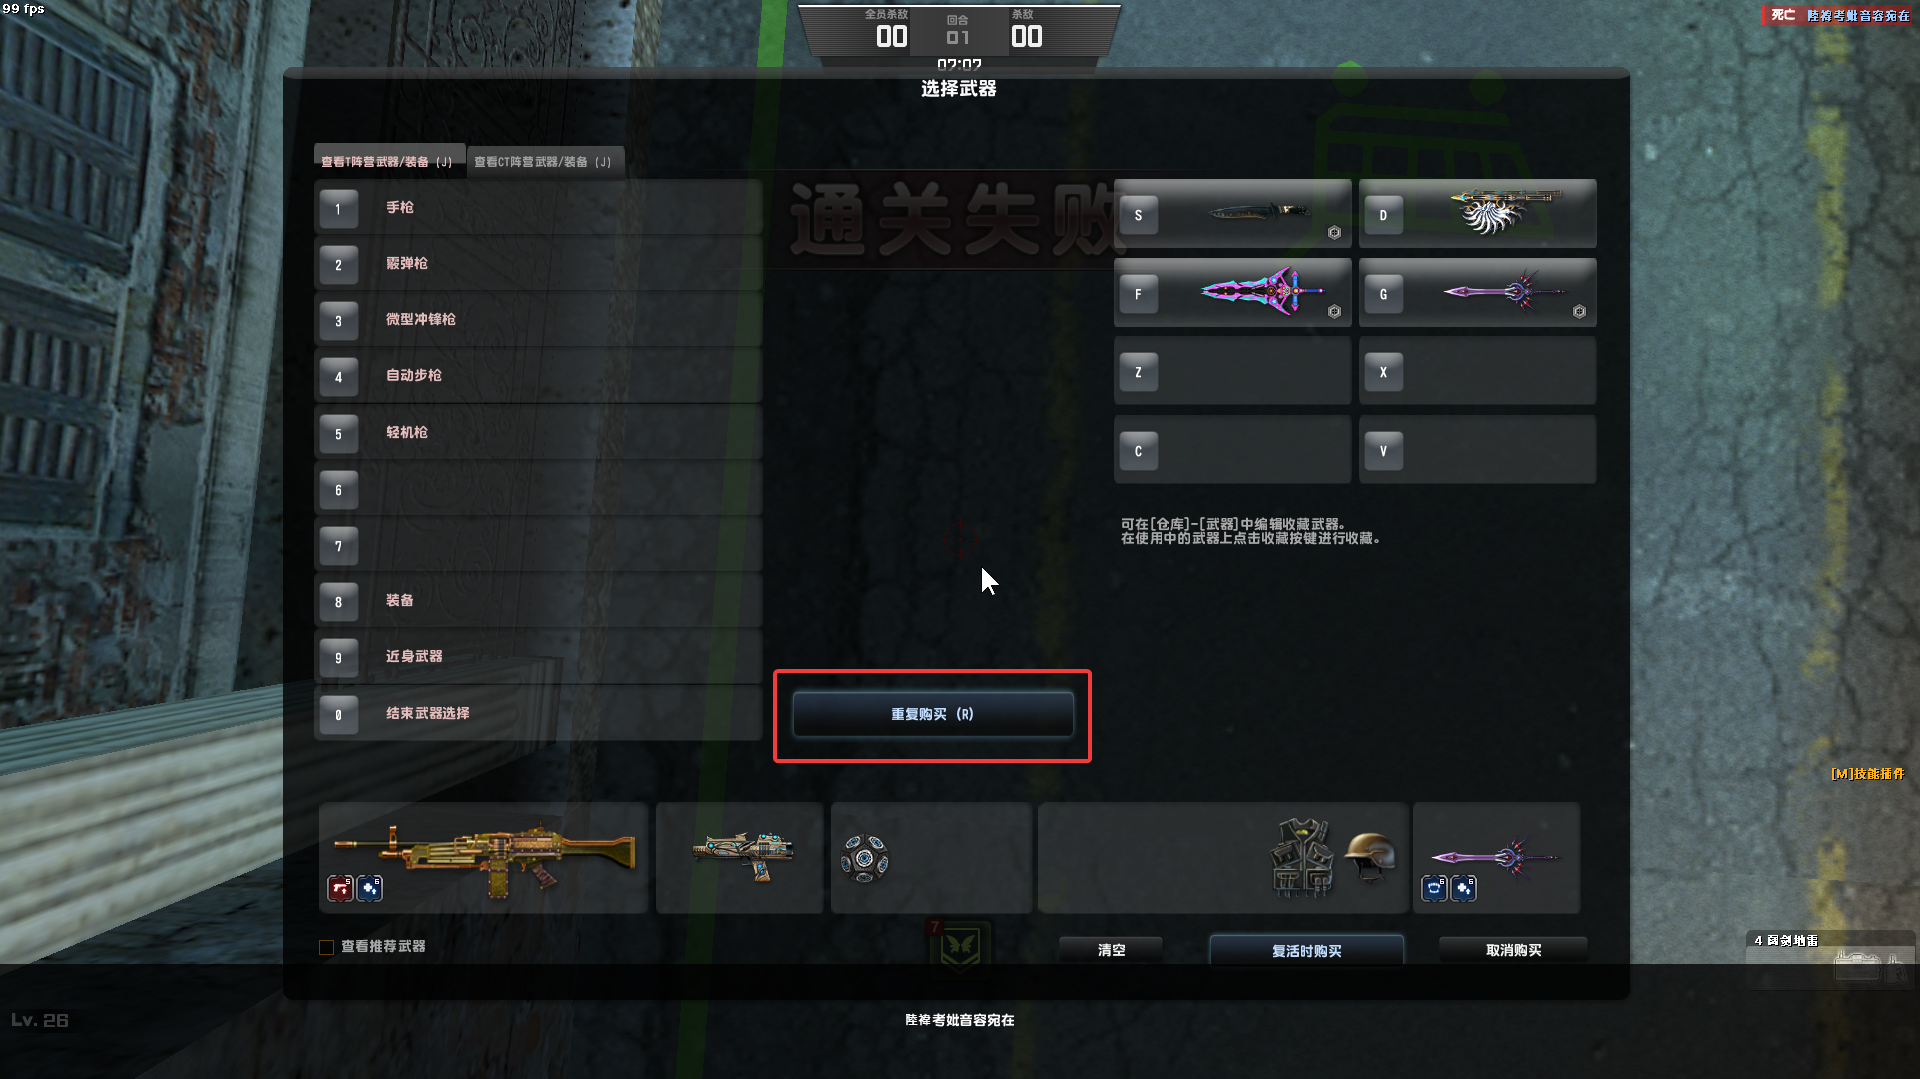
\includegraphics[width=\textwidth]{docs/assets/dead_purchase_rebuy.png}
    \caption{死亡时预购买界面中的“重复购买按钮”}
    \label{ch2fig-dead-purchase-rebuy}
\end{figure}

\begin{figure}[H]
    \Centering
    \parbox[l]{\textwidth}{\lstinline{GAME_ROUND_CONFIRM_X}、\lstinline{GAME_ROUND_CONFIRM_Y}:游戏结算界面的“确认”按钮坐标(图 \ref{ch2fig-confirm-round})。}
    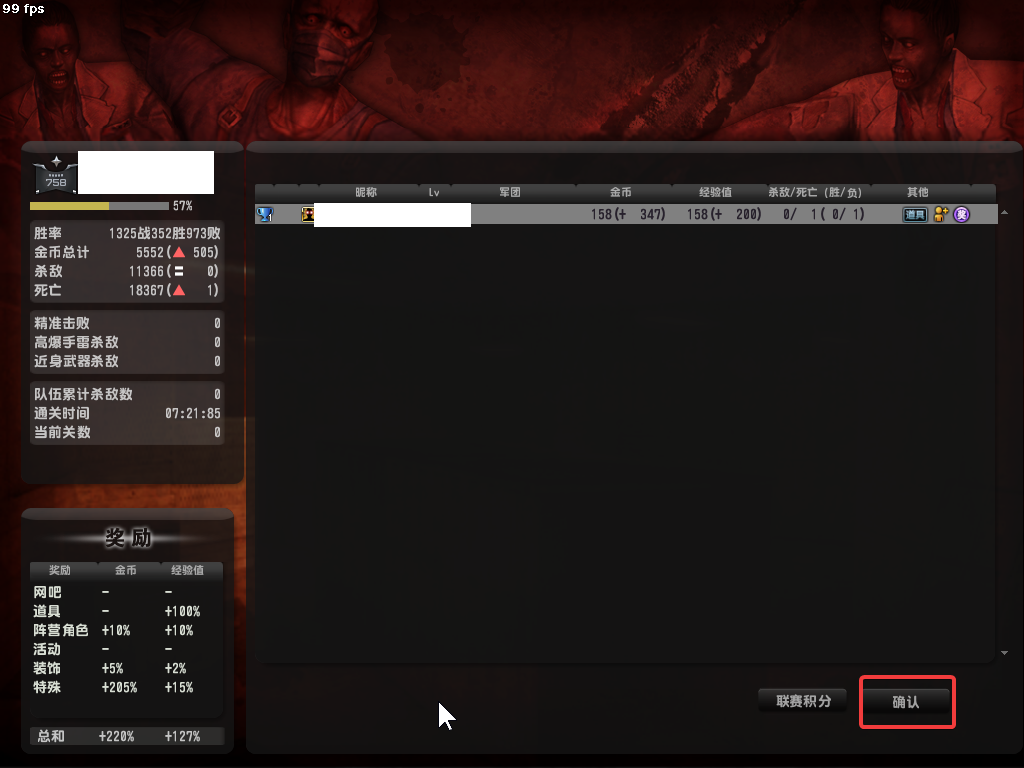
\includegraphics[width=\textwidth]{docs/assets/confirm_round.png}
    \caption{结算界面“确认”按钮}
    \label{ch2fig-confirm-round}
\end{figure}

v1.3.14 引入了创建房间时的锁房功能,锁房可防止有人进入房间恶意举报。

\begin{figure}[H]
    \Centering
    \parbox[l]{\textwidth}{\lstinline{ROOM_USE_PASSWORD_X}、\lstinline{ROOM_USE_PASSWORD_Y}:启用密码的选框坐标(图 \ref{ch2fig-use-password})。}
    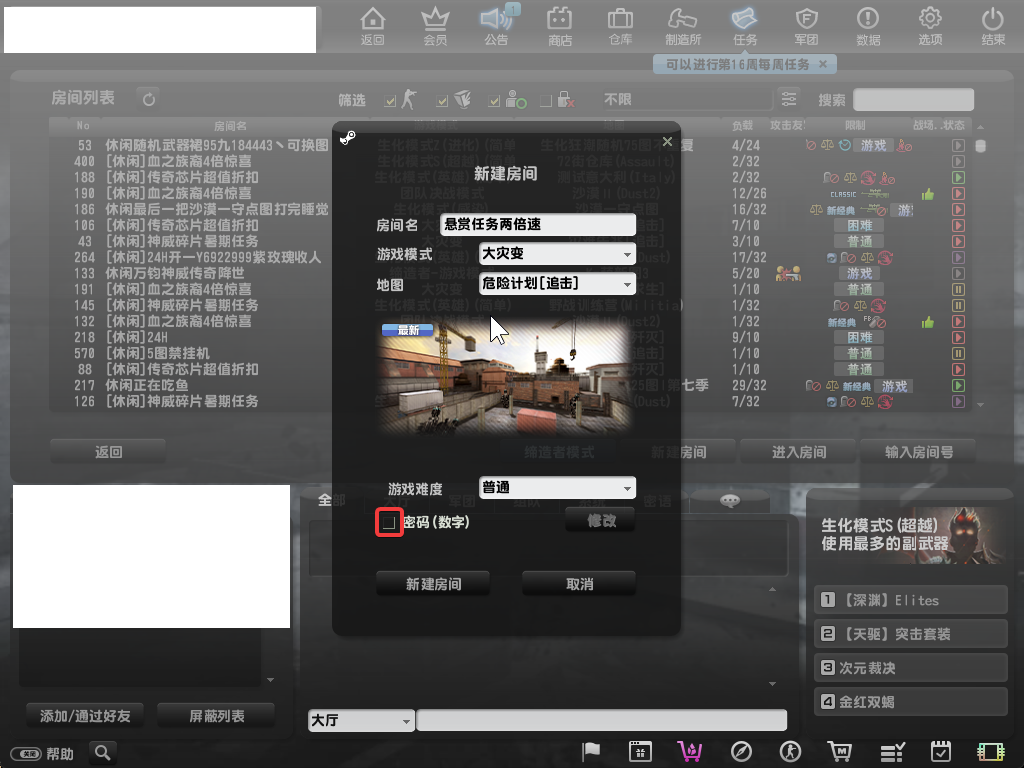
\includegraphics[width=\textwidth]{docs/assets/use_password.png}
    \caption{启用密码功能选框}
    \label{ch2fig-use-password}
\end{figure}

\begin{figure}[H]
    \Centering
    \parbox[l]{\textwidth}{\lstinline{ROOM_PASSWORD_BOX_X}、\lstinline{ROOM_PASSWORD_BOX_Y}:密码输入框坐标(图 \ref{ch2fig-password-box})。}
    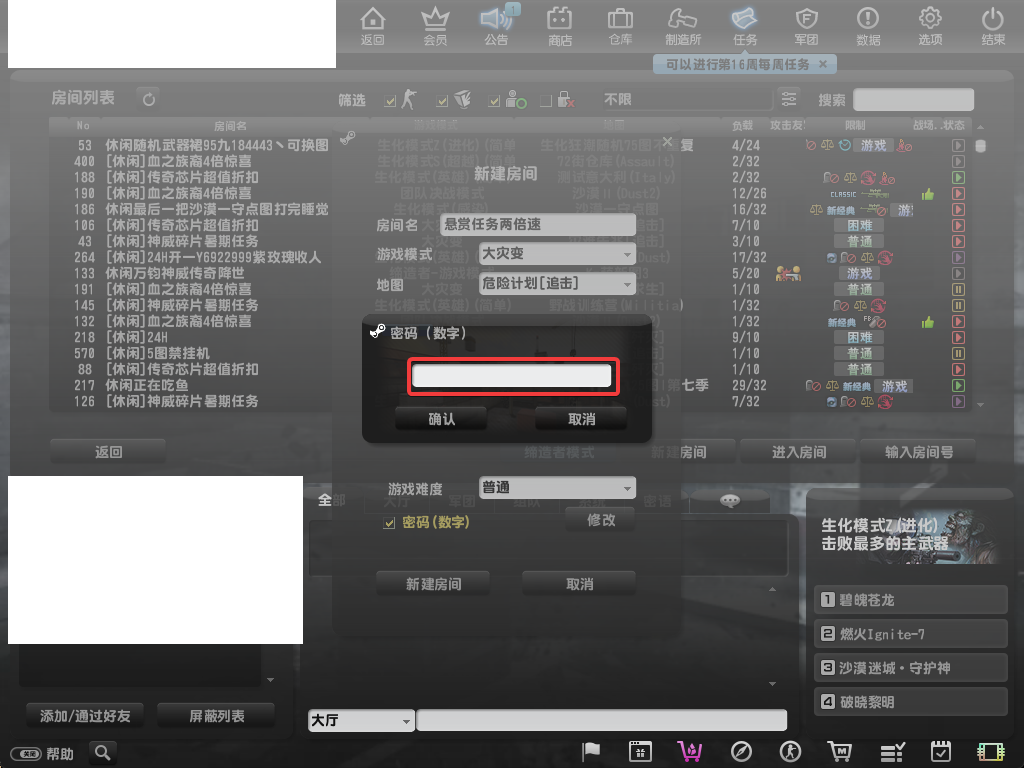
\includegraphics[width=\textwidth]{docs/assets/password_box.png}
    \caption{密码输入框}
    \label{ch2fig-password-box}
\end{figure}

\begin{figure}[H]
    \Centering
    \parbox[l]{\textwidth}{\lstinline{ROOM_PASSWORD_CONFIRM_X}、\lstinline{ROOM_PASSWORD_CONFIRM_Y}:确认密码按钮(图 \ref{ch2fig-confirm-password})。}
    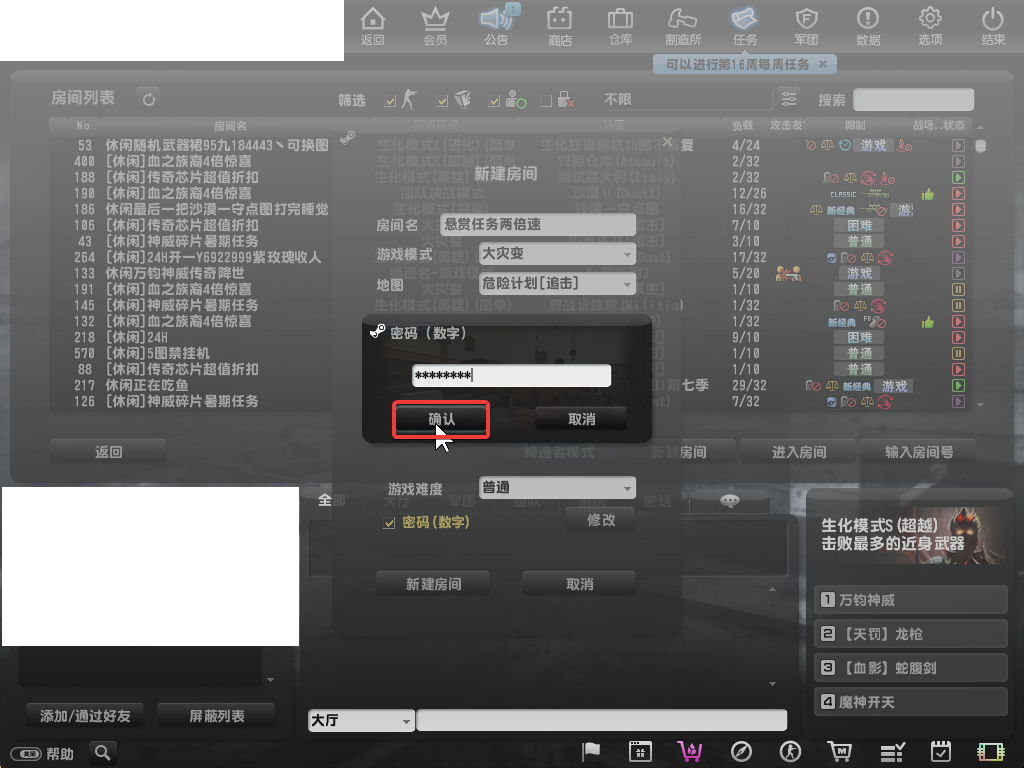
\includegraphics[width=\textwidth]{docs/assets/confirm_password.png}
    \caption{密码输入框}
    \label{ch2fig-confirm-password}
\end{figure}

\lstinline{ROOM_USE_CUSTOM_PASSWORD}:设置为\lstinline{false} 时,将随机生成 8 \textasciitilde 16 位数字密码输入密码框(默认);设置为 \lstinline{true} 时,则使用您指定的密码。

\lstinline{ROOM_CUSTOM_PASSWORD}:房间的自定义密码(\lstinline{ROOM_USE_CUSTOM_PASSWORD} 设置为 \lstinline{true} 时启用),由大小写英文字母及数字构成(若包含其他符号,则这些符号在输入密码时会被忽略)。

\subsection{挂机武器列表}

打开 \lstinline{WeaponList.lua} 文件。文件中已经提供了大量样例,根据下述的说明仔细修改即可。

\subsubsection{默认挂机模式}

1 号模式挂机为默认挂机模式,该模式下玩家会购买配件武器列表中的配件武器辅助并使用默认武器列表中的武器攻击。此模式正常工作需要设置 \lstinline{PartWeaponList}(配件武器列表)和 \lstinline{DefaultWeaponList}(默认武器列表)。
武器列表不限制武器数量,但还是建议根据下文中的建议数量进行设置。

\lstinline{PartWeaponList} 是挂机过程中需要购买的配件武器,配件武器购买后仅用作辅助,不会切换出来使用。

配件武器列表 \lstinline{PartWeaponList} 格式如下(所有的标点符号\textbf{\color{red}必须}为英文标点符号,下同),每件武器都通过 \lstinline|Weapon:new({...})| 创建,您可以仿照样例文件自行创建和删除武器。

\begin{minted}[breaklines, breakautoindent=true]{lua}
PartWeaponList = {
    Weapon:new({
        name = "星战前线·加特林",
        number = Weapon.PRIMARY,
        purchase_sequence = {Keyboard.B, Keyboard.J, Keyboard.TWO, Keyboard.FOUR}
    }),
    Weapon:new({
        name = "FNP-45战损版",
        number = Weapon.SECONDARY,
        purchase_sequence = {Keyboard.B, Keyboard.J, Keyboard.ONE, Keyboard.TWO}
    }),
    Weapon:new({
        name = "燃爆Ignite-10",
        number = Weapon.GRENADE,
        purchase_sequence = {Keyboard.B, Keyboard.J, Keyboard.EIGHT, Keyboard.SEVEN}
    })
}
\end{minted}

每添加一款武器(数量任意,鉴于配件武器不会被使用,故没有必要超过 3 个),均需要在列表中新增相应的 \lstinline|Weapon:new({...})| 项,各个项之间用逗号分隔,空白字符不影响文件解析。

下面对创建配件武器的方式详细说明。

\begin{itemize}
\item \lstinline{name} 为武器的名称,需要确保各个武器的名称彼此不同。
\item \lstinline{number} 为武器的序号,可以取:
\lstinline{Weapon.PRIMARY}(主武器)、\lstinline{Weapon.SECONDARY}(副武器)、\lstinline{Weapon.MELEE}(近战武器)、\lstinline{Weapon.GRENADE}(手雷)。
\item \lstinline{purchase_sequence}:武器购买按键序列。注意 \lstinline{Keyboard.J} 键可以切换不同阵营的武器。
例如上面的\textbf{\color{red}燃爆Ignite-10},其购买按键序列被设置为:

\begin{minted}[breaklines, breakautoindent]{lua}
purchase_sequence = {Keyboard.B, Keyboard.J, Keyboard.EIGHT, Keyboard.SEVEN}
\end{minted}

对应于购买按键序列 \textbf{\color{red}B J 8 7}。仿照上面的例子,应该不难自行配置。
\end{itemize}

默认挂机武器列表 \lstinline{DefaultWeaponList} 是挂机过程中购买并使用的武器。
如文件中给出的例子仅包含一件武器\textbf{\color{red}幻境!·光棱剑},这样就可以实现单武器挂机,可用于 24H 纯刀房。
您还可以添加其他的武器,如镰刀、天驱、次元、青鸾等。
\textbf{\color{red} 考虑到默认挂机模式下,配件武器可能已经占用三个武器栏,因此用于攻击的武器最好都属于同类武器(即同为主武器、副武器、近战武器)。}
默认武器除了需要设置 \lstinline{name}、\lstinline{number}、\lstinline{purchase_sequence} 外,还\textbf{\color{red}必须}设置下列字段:

\begin{itemize}
\item \lstinline{switch_delay}(切枪延迟时间):整数,单位为毫秒,自行配置时可以直接写数字。在不做配置的情况下,默认切枪延迟设置为常量 \lstinline{Delay.NORMAL}(100 毫秒)。
\item \lstinline{attack_button}(攻击鼠标按钮):可设置为 \lstinline{Mouse.LEFT}(鼠标左键)、\lstinline{Mouse.MIDDLE}(鼠标中键)、\lstinline{Mouse.RIGHT}(鼠标右键)、\lstinline{Mouse.BACKWARD}(鼠标后退键)、\lstinline{Mouse.FORWARD}(鼠标前进键)。
魔法刀一般使用左键挥砍,因此文件给出的例子中设置为 \lstinline{Mouse.LEFT}。在不做配置的情况下,默认的攻击按钮为左键。
\end{itemize}

\subsubsection{扩展挂机模式}

2 号挂机模式为扩展挂机模式。该模式下玩家会随机购买扩展武器列表中的武器攻击,并使用特殊武器(如圣翼皓印或炽翼魔印)辅助杀敌,适用于野房挂机抢杀敌 MVP 的情形(阅读完本节后可根据需要参考\nameref{section-skills}章节中的\nameref{subsection-mode-2-skill-0}进行设置)。
考虑到购买随机武器需要消耗较多资金,当切换至该模式时,随机武器列表并不会立即启用,而是会在游戏开始后的 120 秒内先使用模式 1 积攒足够资金后再启用随机武器列表。
除了野房抢杀敌 MVP 外,模式 2 非常适合刷狂戮巨蚊、鹞子风筝等活动任务(阅读完本节后可根据需要参考\nameref{section-skills}章节中的\nameref{subsection-mode-2-skill-1}进行设置)。

该模式需要设置 \lstinline{ExtendedWeaponList}(扩展武器列表)和 \lstinline{SpecialWeapon}(某一件特殊武器,不是列表)。
\lstinline{ExtendedWeaponList} 为扩展武器列表,不限制武器数量,挂机时随机从中抽取武器进行攻击,其配置方式同 \lstinline{DefaultWeaponList},您可以根据提供的样例自行修改。

\lstinline{SpecialWeapon} 为特殊武器,如圣翼皓印或炽翼魔印。\textbf{\color{red} 如您没有特殊武器,只需要将文件中红框部分的短横线删除即可}(图 \ref{ch2fig-delete-special-weapon})。

\begin{figure}
    \Centering
    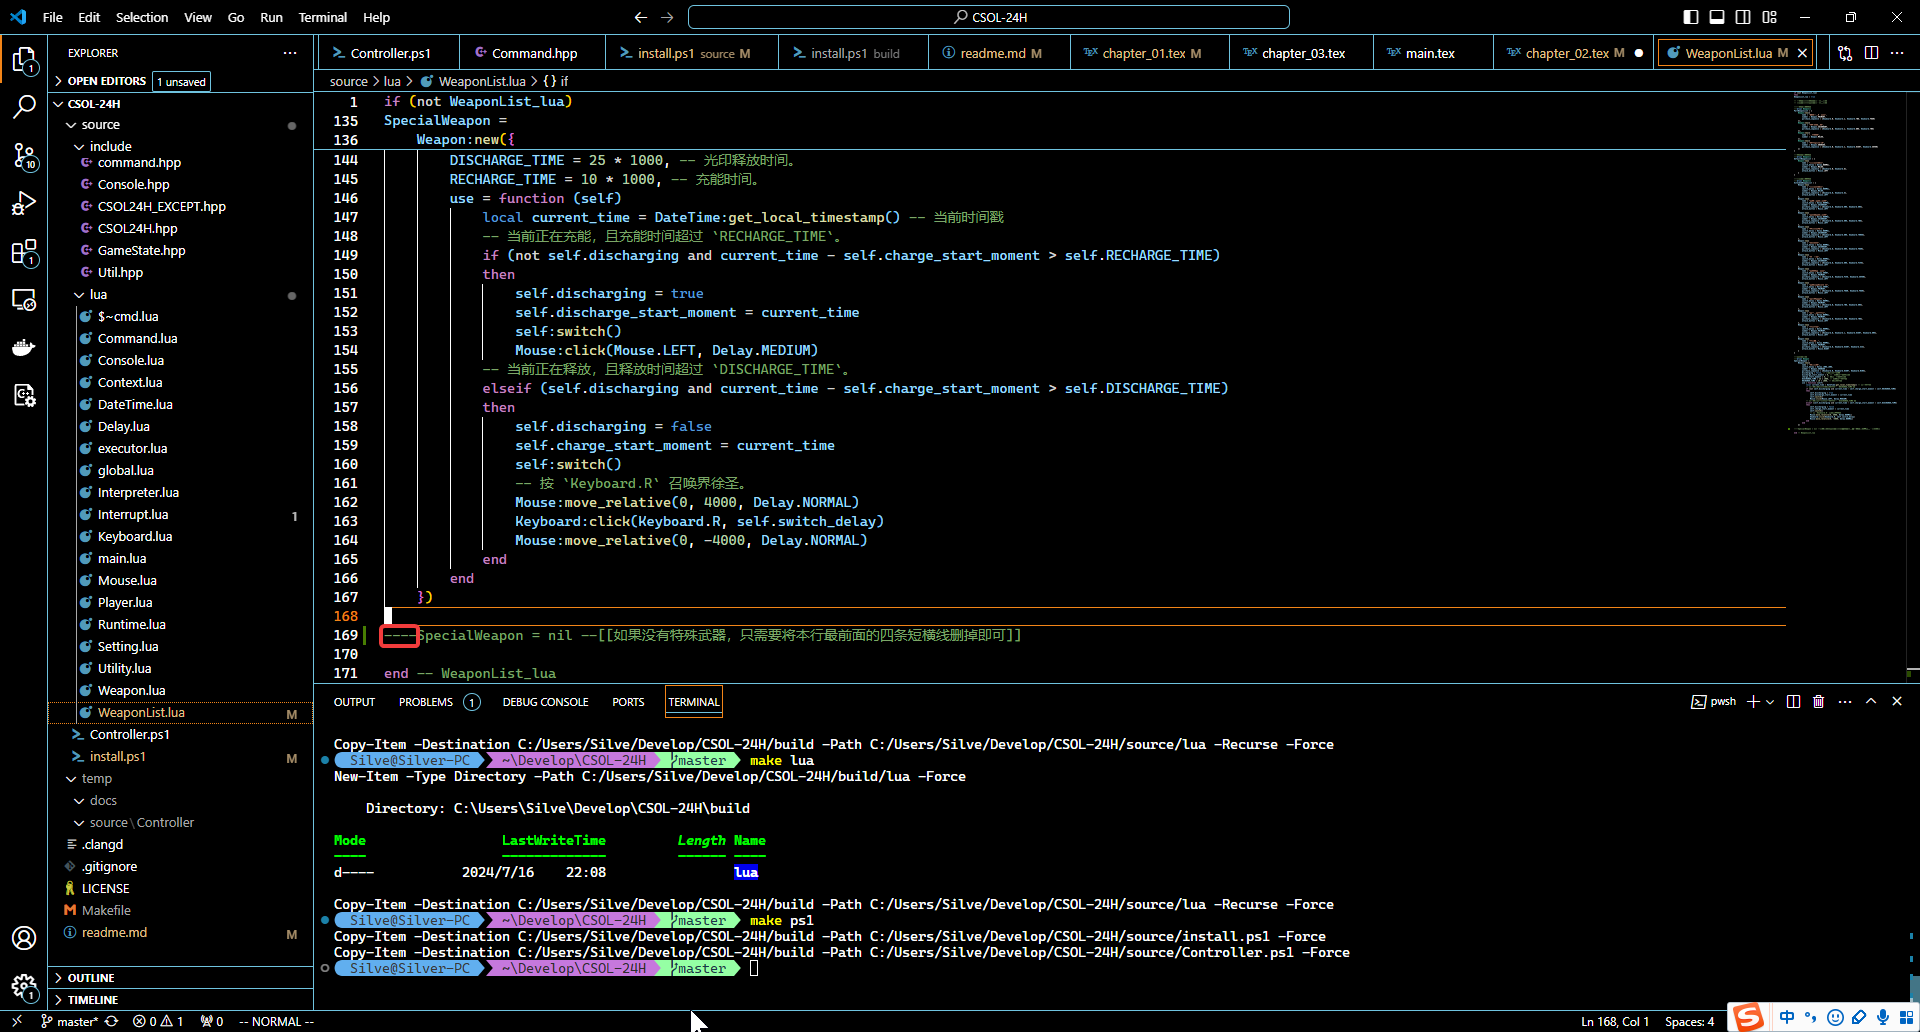
\includegraphics[width=\textwidth]{docs/assets/delete_SpecialWeapon.png}
    \caption{不使用特殊武器}
    \label{ch2fig-delete-special-weapon}
\end{figure}

\textbf{\color{red} 在提供的 \lstinline{WeaponList.lua} 样例文件中,已经编写好了圣翼皓印(或炽翼魔印)使用的方式,如需使用特殊武器,只需要将其中的 \lstinline{purchase_sequence} 修改为自己使用的购买按键序列即可。}
对于有一定编程基础的玩家,可以自定义 \lstinline{SpecialWeapon},重写 \lstinline{use} 方法。
游戏过程中会通过调用 \lstinline{use} 方法使用该特殊武器。

v1.3 中引入了护甲自动购买功能,可大大减少挂机过程中受到的伤害。在 \lstinline{WeaponList.lua} 中找到 \lstinline{AC}, 根据自身情况修改购买按键序列即可使用。

\begin{figure}
    \Centering
    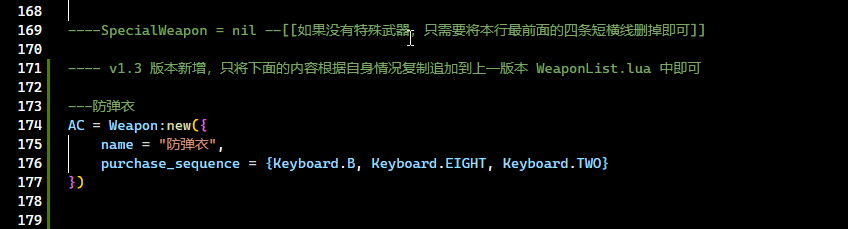
\includegraphics[width=\textwidth]{docs/assets/buy_ac.png}
    \caption{购买护甲}
\end{figure}

如果您的装备购买列表已满,无法通过设置按键的方式购买护甲,则可以将购买队列设置为重复购买按键(游戏内默认设置为 \lstinline{F2}),游戏内重复购买操作将会自动购买小甲(没有头盔)。

\begin{minted}[breakautoindent, breaklines]{lua}
AC = Weapon:new({
    name = "防弹衣+头盔",
    purchase_sequence = {Keyboard.F2}
})
\end{minted}

如果不需要购买护甲(不推荐),则将文件中红框部分的短横线删除即可(图 \ref{ch2fig-delete-ac})。

\begin{figure}
    \Centering
    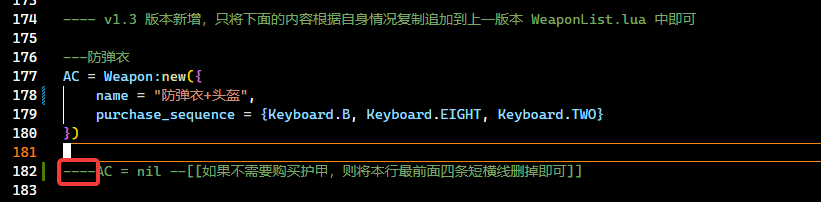
\includegraphics[width=\textwidth]{docs/assets/delete_AC.png}
    \caption{禁用护甲自动购买功能}
    \label{ch2fig-delete-ac}
\end{figure}

\subsection{使用方法}

上述配置无误后,进入一个挂机房间,按 \lstinline{Ctrl} \lstinline{Alt} \lstinline{Shift} \lstinline{1} 或 \lstinline{Ctrl} \lstinline{Alt} \lstinline{Shift} \lstinline{2} 选择 1 模式或 2 模式开始挂机。
对于模式 2,随机购买武器挂机功能将于 120 秒后有充足资金时启用。

在游戏因诸种原因掉线或闪退后,将自动尝试重启游戏,创建地狱围栏房间挂机。该功能无需配置。